\documentclass[thesis2.tex]{subfiles}

\begin{document}
\iffulldocument\else
	\chapter{Chen-McKenna suspension bridge equation}
\fi

This is work done in collaboration with Todd Kapitula (Calvin College) and has been published in preprint form in \cite[Secton 6]{kapitula2019}. Theorems involving the Hamiltonian-Krein index are due to Todd Kapitula; for their proofs, we will cite the appropriate result from \cite{kapitula2019}.

\section{Background}

In 1938, R. G. Cone, the chief engineer of the Golden Gate Bridge, observed that ``a wind of unusual high velocity was blowing through the Golden Gate with the direction normal to the axis of the bridge... the suspended structure of the bridge was undulating vertically in a wavelike motion of considerable amplitude'' \cite{McKenna1990}. Motivated by observations of traveling waves on suspension bridges, McKenna and Walter \cite{McKenna1990} proposed the model,
\begin{equation}\label{susp}
\partial_t^2u + \partial_x^4u + u^+ - 1 = 0,
\end{equation}
to describe waves propagating on an infinitely long suspended beam, where $u^+ = \max(u, 0)$. The beam bends under its own weight, and the term $u^+$ represents the restoring force. Since the beam is suspended from above, the restoring force is one-sided since it only counteracts downward deflections. To reduce the complexity due to the nonsmooth term $u^+$, Chen and McKenna \cite{Chen1997} introduced the regularized equation,
\begin{equation}\label{susp2}
\partial_t^2u + \partial_x^4u + \rme^{u-1} - 1 = 0.
\end{equation}
Making the change of variables $u - 1 \mapsto u$ in \cref{susp2}, so that localized solutions will decay to a baseline of 0, we will consider the equation,
\begin{equation}\label{susp3}
\partial_t^2u + \partial_x^4u +  \rme^{u} - 1 = 0.
\end{equation}
Writing this in a co-moving frame with speed $c$ by letting $\xi = x - ct$, equation \cref{susp3} becomes
\begin{equation}\label{suspc}
\partial_t^2u - 2 c\partial_{xt}^2u +\partial_x^4u +  c^2\partial_x^2u + \rme^{u} - 1 = 0,
\end{equation}
where we have renamed the independent variable back to $x$.

An equilibrium solution to \cref{suspc} satisfies the ODE,
\begin{equation}\label{CheneqODE}
\partial_x^4u +  c^2\partial_x^2u + \rme^{u} - 1 = 0.
\end{equation}
Smets and van den Berg \cite[Theorem 11]{Smets2002} prove the existence of a localized, symmetric solution $U(x)$ to \cref{CheneqODE} for almost all wavespeeds $c \in (0, \sqrt{2})$. van den Berg et.al. \cite[Theorem~1]{Berg2018} use a computer-assisted proof technique to show existence of such solutions to \cref{CheneqODE} for all speeds $c$ with $c^2 \in [0.5, 1.9]$. We take the following hypothesis.

\begin{hypothesis}\label{Uexistshyp}
An exponentially localized primary pulse solution $U(x; c)$ exists to \cref{CheneqODE} for each wavespeed $c \in (0, \sqrt{2})$ and is smooth in the wavespeed.
\end{hypothesis}

For the remainder of this section, we will fix $c \in (0, \sqrt{2})$ and write the primary pulse solution corresponding to wavespeed $c$ as $U(x)$. We are interested in the existence and stability of multi-pulse equilibrium solutions to \cref{suspc}. A multi-pulse is a localized, multi-modal solution $U_n(x)$ to \cref{CheneqODE} which resembles multiple, well-separated copies of the primary pulse $U(x)$.

\section{Existence of pulses}

First, we look at the existence of such pulses. The linearization of \cref{CheneqODE} about a given solution $U_*$ of \cref{CheneqODE} is,
\begin{equation}\label{defA0}
\calA_0(U^*) = \partial_x^4 + c^2 \partial_x^2 + \rme^{U_*}.
\end{equation}
We take the following hypothesis concerning $\calA_0(U)$.

\begin{hypothesis}\label{A0hyp}
On the space $L^2(\R)$, the point spectrum of $\calA_0(U)$ consists of exactly two eigenvalues:
\begin{enumerate}
\item $\calA_0(U)$ has a one-dimensional kernel spanned by $\partial_x U(x)$.
\item $\rmn[\calA_0(U)]=1$, i.e. $\calA_0(U)$ has a unique, simple negative eigenvalue $\lambda_-$.
\end{enumerate}
\end{hypothesis}

\begin{remark}While the results below hold if we only make assumptions on the nonnegative point spectrum of $\calA_0(U)$, \cref{A0hyp} is supported by numerical evidence. For simplicity, we make assumptions on the entire point spectrum of $\calA_0(U)$.
\end{remark}

From this hypothesis, it follows that the primary pulse $U(x)$ is transversely constructed in the ODE phase space. Before stating our theorem, we will also need the following result. For $c \in (0, \sqrt{2})$, the solutions to the constant-coefficient equation,
\[
\calA_0(0)v = \partial_x^4 v + c^2 \partial_x^2 v + 1 = 0,
\]
are given by $v = \rme^{\mu x}$, where
\begin{align}\label{specA00}
\mu = \pm \sqrt{\frac{-c^2 \pm \sqrt{c^4 - 4}}{2} } = \pm \alpha \pm \rmi\beta,
\end{align}
for $\alpha, \beta > 0$. The constant $\alpha$ is the exponential decay rate of localized solutions to \cref{CheneqODE}. We now have the following theorem, which is adapted from \cite[Theorem~3.6]{SandstedeStrut}. In all that follows, the norm $||\cdot||_\infty$ is the supremum norm on $C(\R)$ and $\langle \cdot, \cdot \rangle$ is the inner product on $L^2(\R)$.

\begin{theorem}\label{multiexist}
Assume Hypothesis \ref{Uexistshyp} and Hypothesis \ref{A0hyp}. Fix a wavespeed $c$, and let $U(x)$ be an exponentially localized solution to \cref{CheneqODE}. Then for any $n \geq 2$ and any sequence of nonnegative integers $k_1, \dots, k_{n-1}$ with at least one of the $k_j \in \{0, 1 \}$, there exists a nonnegative integer $m_0$ and $\delta > 0$ such that:
\begin{enumerate}%[(i)]
	\item For any integer $m$ with $m \geq m_0$, there exists a unique $n-$modal solution $U_n(x)$ to \cref{CheneqODE} which is of the form
	\begin{equation}\label{qn}
	U_n(x) = \sum_{j = 1}^{n} U^j(x) + r(x),
	\end{equation}
	where each $U^j(x)$ is a translate of the primary pulse $U(x)$. The distance between the peaks of $U^j$ and $U^{j+1}$ is $2 X_j$, where
	\begin{equation*}
	X_j \approx \frac{\pi}{\beta}(2 m + k_j) + \tilde{X},
	\end{equation*}
	$\beta$ is defined in \cref{specA00}, and $\tilde{X}$ is a constant. The remainder term $r(x)$ satisfies
	\begin{equation}\label{rbound}
	\|r\|_\infty \leq C \rme^{-\alpha X_{\mathrm{min}}},
	\end{equation}
	where $\alpha$ is defined in \cref{specA00}, and $X_{\mathrm{min}} = \min\{X_1, \dots, X_{n-1}\}$. This bound holds for all derivatives with respect to $x$.

	\item The point spectrum of the linear operator $\calA_0(U_n)$ on $L^2(\R)$ consists of exactly $2n$ eigenvalues, which are as follows:
  \begin{enumerate}
    \item There are $n$ real eigenvalues $\nu_1, \dots, \nu_n$ with $|\nu_j| < \delta$, where $\nu_n = 0$ is a simple eigenvalue, and for $j = 1, \dots, n-1$,
    \[
  	\begin{array}{l}
  	\nu_j < 0 \text{ if } k_j \text{ is odd} \\
  	\nu_j > 0 \text{ if } k_j \text{ is even.}
  	\end{array}
    \]
    We will refer to these as the small magnitude eigenvalues of $\calA_0(U_n)$. For $j = 1, \dots, n-1$, $\nu_j = \mathcal{O}(\rme^{-2\alpha X_{\mathrm{min}}})$, and the corresponding eigenfunctions $s_j$ are given by
  	\begin{equation}\label{sj}
  	s_j = \sum_{k = 1}^{n} d_{jk}\partial_x U^k + w_j,
  	\end{equation}
  	where $d_{jk} \in \C$ are constants, and the remainder terms $w_j$ satisfy
  	\begin{equation}\label{sjwbound}
  	\|w_j\|_\infty \leq C\rme^{-2 \alpha X_{\mathrm{min}}}.
  	\end{equation}
    This bound holds for all derivatives with respect to $x$. The eigenfunction corresponding to $\nu_n$ is $s_n = \partial_x U_n$.

    \item There are $n$ negative eigenvalues which are $\delta-$close to $\lambda_-$.
  \end{enumerate}

  \item The essential spectrum of $\calA_0(U)$ is
    \begin{equation}\label{A0ess}
    \sigma_{\text{ess}}(\calA_0(U)) = [1 - c^4/4, \infty).
    \end{equation}
    which is positive and bounded away from 0.

\end{enumerate}
\end{theorem}

\begin{proof}
Equation \cref{CheneqODE} is Hamiltonian with energy
\begin{equation}\label{defH}
H(u) = \left(\partial_xu\right)\left(\partial_x^4 u\right) - \frac{1}{2}\left(\partial_x^2u\right)^2 + \frac{c^2}{2}\left(\partial_xu\right)^2 + \rme^u - u.
\end{equation}
Using \cref{specA00}, \cref{defH}, the assumption that the kernel is simple, and the fact that the Melnikov integral $M = \int_{-\infty}^\infty (\partial_x U)^2\,\rmd x$ is positive, (a) follows from \cite[Theorem~3.6]{SandstedeStrut}, except for the bound on $r(x)$, which follows from \cite{Sandstede1993} and \cite{Sandstede1998}. All eigenvalues are real since $\calA_0(U_n)$ is self-adjoint on $L^2(\R)$.  From Hypothesis \ref{A0hyp}, $\calA_0(U)$ has a simple eigenvalue at 0 and a simple negative eigenvalue at $\lambda_-$. It follows from \cite{Alexander1990} that $\calA_0(U_n)$ has exactly $n$ eigenvalues near each eigenvalue of $\calA_0(U)$, i.e. $n$ eigenvalues near 0 and $n$ negative eigenvalues near $\lambda_-$. This proves the eigenvalue count and part (b2). Part (b1) follows from \cite{Sandstede1998}. We can verify directly that $\calA_0(U_n)\partial_x U_n = 0$. Part (c) follows from the Weyl Essential Spectrum Theorem \cite[Theorem~2.2.6]{Kapitula2013} and \cite[Theorem~3.1.11]{Kapitula2013}, since $\calA_0(U_n)$ is exponentially asymptotic to $\calA_0(0)$.
\end{proof}

\section{Stability of pulses}

Now that we know about the existence of single and multiple pulses, we consider their spectral stability. To determine linear PDE stability of the multi-pulse solutions constructed in Theorem \ref{multiexist}, we look at the linearization of the PDE \cref{suspc} about $U_n(x)$, which is the quadratic operator polynomial $\calP_2(\lambda; U_n): H^4(\R, \C) \subset L^2(\R,\C) \rightarrow L^2(\R,\C)$ given by
\begin{equation}\label{quadeig}
\calP_2(\lambda; U_n) = \calI \lambda^2 + \calA_1 \lambda + \calA_0(U_n)
\end{equation}
where $\calA_0(U_n)$ is defined in \cref{defA0}, $\calI$ refers to the identity, and $\calA_1=-2 c \partial_x$.

First, we consider the essential spectrum. Since $U_n$ is exponentially localized, $\calP_2(\lambda; U_n)$ is exponentially asymptotic to the operator
\begin{equation}\label{quadeig0}
\calP_2(\lambda; 0) = \partial_x^4 + c^2 \partial_x^2 - 2 c \lambda \partial_x + (\lambda^2 + 1).
\end{equation}
By \cite[Theorem~3.1.11]{Kapitula2013}, $\calP_2(\lambda; U_n)$ is a relatively compact perturbation of $\calP_2(\lambda; 0)$, thus by the Weyl essential spectrum theorem \cite[Theorem~2.2.6]{Kapitula2013}, $\calP_2(\lambda; U_n)$ and $\calP_2(\lambda; 0)$ have the same essential spectrum. To find the essential spectrum of $\calP_2(\lambda; 0)$, consider the related first-order operator $\calT(\lambda): H^1(\R, \C^4) \subset L^2(\R,\C^4) \rightarrow L^2(\R,\C^4)$ given by
\begin{equation}
\calT(\lambda) = \frac{\rmd}{\rmd x} - \begin{pmatrix}
0 & 1 & 0 & 0 \\
0 & 0 & 1 & 0 \\
0 & 0 & 0 & 1 \\
-1 - \lambda^2 & 2 c \lambda & -c^2 & 0
\end{pmatrix},
\end{equation}
which we obtain by writing $\calP_2(\lambda; 0)$ as a first order system. By a straightforward adaptation of \cite[Theorem A.1]{SanScheel2007} (the only difference being the presence of the fourth-order differential operator), the operators $\calT(\lambda)$ and $\calP_2(\lambda; 0)$ have the same Fredholm properties, thus the same essential spectrum. By a straightforward calculation,
\begin{equation}\label{quadess}
\sigma_{\mathrm{ess}}(\calP_2(\lambda; U_n)) = \sigma_{\mathrm{ess}}(\calT(\lambda)) = \{\rmi r : |r| \geq \rho \},
\end{equation}
where $\rho > 0$ is the minimum of the function $\lambda(r) = c r + \sqrt{1 + r^4}$. The value of $\rho$ is positive for $c \in (0, \sqrt{2})$, and $\rho\to 0$ as $c\to\sqrt{2}$, as shown in \cref{fig:essspecrho}. Since the essential spectrum is purely imaginary and bounded away from 0, spectral stability thus depends entirely on the point spectrum.
\begin{figure}
\centering
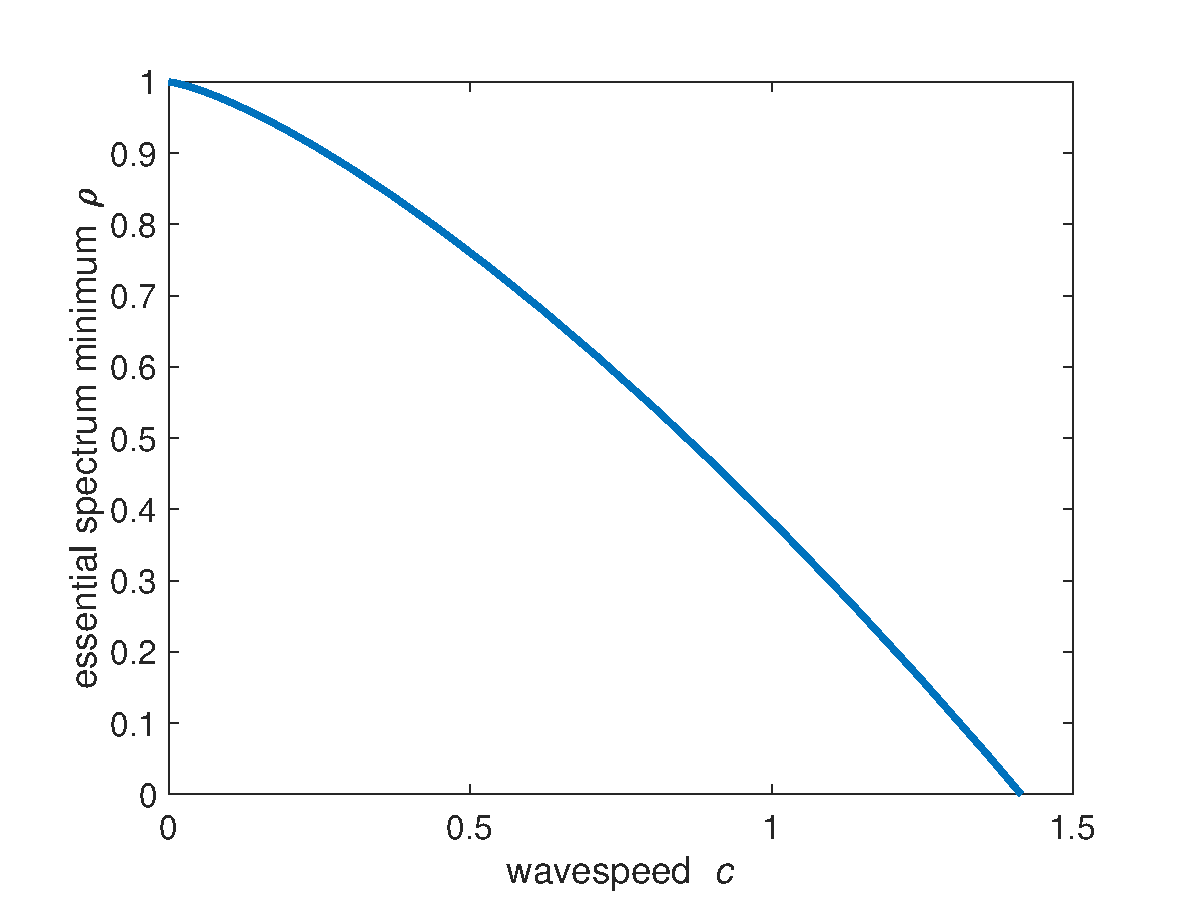
\includegraphics[width=8cm]{images/chen/essspecrho.eps}
\caption[Essential spectrum bound for Chen-McKenna]{Minimum of purely imaginary essential spectrum $\rho$ vs. wavespeed $c$.}
\label{fig:essspecrho}
\end{figure}

\subsection{Single pulse}

Before considering the spectral stability of the $n$-pulse, we must show the stability of the primary pulse, $U(x)$. In addition to Hypothesis \ref{Uexistshyp} and Hypothesis \ref{A0hyp}, our assumptions are:

\begin{hypothesis}\label{PDEexisthyp}
Regarding the PDE \cref{suspc} and the base solution $U(x)$,
\begin{enumerate}
  \item for every initial condition $u(x,0)$ and $\partial_tu(x,0)$ there exists a solution $u(x, t)$ to \cref{suspc} on the interval $I = [0, T]$, where
      \[
      T=T\left(\max\{ ||u(x,0)||, ||\partial_tu(x,0)|| \}\right)
      \]
  \item the constrained energy evaluated on the wave, $d(c)$ (see \cite[Equation~(2.16)]{Grillakis1987} for the exact expression), is concave up,
\begin{equation}\label{dcc}
d''(c) = -\partial_c\left( c\|\partial_xU\|^2 \right)>0,\quad0<c^2<2.
\end{equation}
\end{enumerate}
\end{hypothesis}
We will provide numerical evidence that these hypotheses are met in \cref{sec:numerics}.

Under these assumptions, we will prove the spectral and orbital stability of the single pulse using the Hamiltonian-Krein index (HKI). Briefly, the HKI counts the potentially unstable eigenvalues. The HKI is defined to be the sum of the three indices,
\[
K_{\Ham}=k_\rmr+k_\rmc+k_\rmi^-, 
\]
where $k_\rmr$ is the total number (counting multiplicity) of real and positive eigenvalues, $k_\rmc$ is the total number (counting multiplicity) of eigenvalues with positive real part and nonzero imaginary part, and $k_\rmi^-$ is the total negative Krein index of all purely imaginary eigenvalues. If the imaginary eigenvalues are simple, $k_\rmi^-$ is the total number (counting multiplicity) of nonzero, purely imaginary eigenvalues with negative Krein signature. This last group of eigenvalues is potentially unstable, since collisions between imaginary eigenvalues of opposite Krein signature generically lead to a Hamiltonian-Hopf bifurcation; when this occurs, both eigenvalues leave the imaginary axis in opposite directions, creating an unstable eigenvalue \cite[Chapter 7.1]{Kapitula2013}. 

Before we can use the HKI, there are two issues that must be resolved. First, the HKI as forumulated in \cite{kapitula2019} assumes that $\calA_0$ has a compact resolvent, which is certainly not true for the operator associated with this problem. This compactness assumption is taken primarily for the sake of convenience, and to remove the possibility of point spectrum being embedded in the essential spectrum. However, as seen in the original formulation of the HKI for solitary waves, see \cite{Kapitula2004}, this is not a necessary condition. It is sufficient to assume that the origin is an isolated eigenvalue, and $\calA_0$ is a higher-order differential operator than $\calA_1$ with $\rmn[\calA_0]<+\infty$. The second difficulty is that these previous results for solitary waves do not immediately apply to quadratic eigenvalue problems.  However, as seen in \cite[Section~4.1]{Bronski2014} one can easily convert a quadratic eigenvalue problem into a linear star-even eigenvalue problem, and then apply the index theory to the reformulated problem. Thus, we can conclude the index theory is applicable to the problem at hand, which allows for the following stability result.

\begin{lemma}\label{qstable}
Let $c^2 \in (0, 2)$, and let $U(x)$ be the primary pulse solution to \cref{CheneqODE}. Then $U(x)$ is spectrally and orbitally stable if and only if
\[
d''(c) = -\partial_c\left( c\|\partial_xU\|^2 \right)>0,
\]
where $d(c)$ is defined in \cite[equation (2.16)]{Grillakis1987}.
\end{lemma}

\begin{proof}
We first check that the origin is an isolated eigenvalue. The essential spectrum of $\calA_0(U)$ is the same as that of $\calA_0(U_n)$, and is given by \cref{A0ess}, which is positive and bounded away from 0. By assumption, $\calA_0(U)$ has a single negative eigenvalue. The proof is then completed using the HKI, following the proof of \cite[Lemma 6.6]{kapitula2019}.
\end{proof}

\subsection{$n$-pulse}

We now locate all potentially unstable eigenvalues of \cref{quadeig} for an $n$-pulse. These include polynomial eigenvalues with positive real part, as well as purely imaginary polynomial eigenvalues with negative Krein signature. To accomplish this task we use the HKI in combination with the Krein matrix. First, we compute the HKI for \cref{quadeig}, so that  we have an exact count of the number of potentially unstable polynomial eigenvalues. We then use the Krein matrix to find $(n-1)$ pairs of eigenvalues close to 0; each pair is either real or purely imaginary with negative Krein signature. We refer to these as small magnitude polynomial eigenvalues, or interaction polynomial eigenvalues, since heuristically they result from interactions between neighboring pulses. We then show that the number of potentially unstable interaction polynomial eigenvalues is exactly the same as the HKI, from which we conclude that we have found all of the potentially unstable eigenvalues. By Hamiltonian reflection symmetry, all other point spectrum must be purely imaginary with positive Krein signature.

We start with the calculation of the HKI. By \cref{multiexist} we know that $\calA_0(U_n)$ has precisely $n$ eigenvalues near the origin. Let $0\le n_\rms\le n-1$ represent the number of these eigenvalues which are negative. We have the following result concerning the HKI for the $n$-pulse:

\begin{lemma}\label{lem:HKImulti}
Assume Hypotheses \ref{Uexistshyp}, \ref{A0hyp}, and \ref{PDEexisthyp}, and let $U_n(x)$ be an $n-$modal solution to \cref{CheneqODE}. Then
\[
K_{\Ham}=n+n_\rms-1.
\]
\end{lemma}

\begin{proof}
The proof is given in \cite[Lemma 6.7]{kapitula2019}.
\end{proof}

We now locate the potentially unstable polynomial eigenvalues of the quadratic eigenvalue problem \cref{quadeig}. This will be accomplished through the Krein matrix. Briefly, the Krein matrix is square matrix-valued function $\vK_S(\lambda)$ associated with an eigenvalue problem that has the following properties. For
$\lambda\in\rmi\R$,
\begin{enumerate}
\item $\vK(\lambda)$ is Hermitian and meromorphic
\item $\det\vK(\lambda)=0$ only if $\lambda$ is an  eigenvalue
\item $\vK(\lambda)$ can be used to determine the Krein signature an eigenvalue.
\end{enumerate}
It was first introduced in \cite{Kap2010} and subsequently refined in \cite{kapitula2019} to apply to quadratic eigenvalue problems.

For the sake of exposition only we will henceforth assume that each of the small magnitude eigenvalues $\nu_1, \dots, \nu_n$ of $\calA_0(U_n)$ is simple. For each of these eigenvalues, denote the associated normalized eigenfunctions as $s_1, \dots, s_n$. Since $\calA_0(U_n)$ is self-adjoint, these eigenfunctions are pairwise orthogonal. In the construction of the Krein matrix the relevant subspace for the spectral problem is the span of this set of eigenfunctions associated with the small magnitude eigenvalues of $\calA_0$,
\begin{equation}\label{defS}
S = \Span\{s_1, \dots, s_n \}.
\end{equation}

We now present the following theorem, which is the main result of this section.

\begin{theorem}\label{Kreindiag}
Assume Hypotheses \ref{Uexistshyp}, \ref{A0hyp}, and \ref{PDEexisthyp}. Let $U_n(x)$ be an $n-$pulse solution to \cref{CheneqODE}, and let $\nu_1, \dots, \nu_n$ be the small magnitude eigenvalues of $\calA_0(U_n)$, as defined in \cref{multiexist}. Under a suitable normalization of the eigenfunctions $s_j$, near the origin the Krein matrix has the asymptotic expansion,
\begin{equation}\label{Kreinapprox}
-\frac{\vK_S(z)}{z} = ||\partial_xU||^2 \mathrm{diag} (\nu_1, \dots, \nu_n)
 + d''(c)\vI_n\overline{z}^2 + \mathcal{O}(\rme^{-(3 \alpha/2) X_{\mathrm{min}}}|z| + |z|^3),
\end{equation}
which is diagonal to leading order.
\end{theorem}

The proof of this result is left to \cref{s:kreinproof}. As a corollary, we have the following criteria for spectral stability and instability of the multi-pulse solutions $U_n(x)$.

\begin{corollary}\label{stabcrit}
Let $U_n(x)$ be an $n-$pulse solution to \cref{CheneqODE} constructed as in \cref{multiexist} using the sequence of nonnegative integers $\{ k_1, \dots, k_{n-1} \}$. Assume the same hypotheses as in \cref{Kreindiag}. Let $\nu_1, \dots, \nu_n$ be the small magnitude eigenvalues of $\calA_0(U_n)$, where $\nu_n = 0$. Then there are $(n-1)$ pairs of eigenvalues of \cref{quadeig} close to 0, which we will term interaction polynomial eigenvalues. These are described as follows. For each $j=1,2,\dots,n-1$,
\begin{enumerate}
  \item if $k_j$ is odd (equivalently, $\nu_j<0$), there is a corresponding pair of purely imaginary interaction polynomial eigenvalues,
  \begin{equation}\label{npulseKreineigs}
	\lambda_j^\pm = \pm \rmi \left( \|\partial_xU\| \sqrt{ \frac{|\nu_j|}{d''(c)} } + \mathcal{O}(\rme^{-(3 \alpha/2) X_{\mathrm{min}}}) \right),
	\end{equation}
  each of which has negative Krein signature
  \item if $k_j$ is even (equivalently, $\nu_j>0$), there is a corresponding pair of real interaction polynomial eigenvalues,
   	\[
	\lambda_j = \pm \left( \|\partial_xU\| \sqrt{ \frac{\nu_j}{d''(c)} } + \mathcal{O}(\rme^{-(3 \alpha/2) X_{\mathrm{min}}}) \right).
	\]
  In particular, there exists a positive, real eigenvalue.
\end{enumerate}
In addition, there is a geometrically simple polynomial eigenvalue at $\lambda=0$ with corresponding eigenfunction $\partial_x U_n$. All other point spectra is purely imaginary, and has positive Krein signature.
\end{corollary}

\begin{remark}
In other words, if all the small magnitude eigenvalues of $\calA_0(U_n)$ are negative, and if the individual pulses are sufficiently well-separated, then the $n$-pulse is spectrally stable; otherwise, it is unstable.
\end{remark}

While we can find the interaction polynomial eigenvalues using Lin's method as in \cite{Sandstede1998}, using the Krein matrix allows us to also determine the Krein signatures of any purely imaginary interaction polynomial eigenvalues. This additional information is needed to ensure that via the HKI all of the potentially unstable point spectrum has small magnitude.

\begin{remark}The spectral stability result only holds for sufficiently large $X_{\mathrm{min}}$. In particular, if this is not the case, there may be a Krein collision between an interaction eigenvalue and the essential spectrum.
\end{remark}

\begin{proof}
By \cite[Corollary 5.3]{kapitula2019} the small polynomial eigenvalues are found by solving $\det\vK_S(z) = 0$. This is equivalent to finding zeros of the Krein eigenvalues. For $j=1,2,\dots,n$ set,
\[
-\frac{r_j(z)}{z}=||\partial_xU||^2 \nu_j + d''(c) \overline{z}^2+\tilde{r}_j(z),
\]
where
\[
\tilde{r}_j(z) = \mathcal{O}(\rme^{-(3 \alpha/2) X_{\mathrm{min}}}|z| + |z|^3).
\]
Note that the first two terms in $-r_j(z)/z$ are the diagonal entries of the Krein matrix. Since to leading order the Krein matrix is diagonal,  by \cite{Ipsen2008} these are valid asymptotic expressions for the Krein eigenvalues. The small and nonzero polynomial eigenvalues are found by solving,
\begin{equation}\label{eqforz}
||\partial_xU||^2 \nu_j + d''(c) \overline{z}^2+\tilde{r}_j(z)=0,\quad j=1,2,\dots,n.
\end{equation}

First suppose that $z$ is real, so the Krein matrix is Hermitian. The Krein eigenvalues are then real-valued; in particular, the error term, $\tilde{r}_j(z)$, is real-valued. Recall that $d''(c)>0$. Suppose that $\nu_j<0$, and set,
\begin{equation}\label{epsilon2}
\epsilon_j^2 = -\frac{||\partial_xU||^2 \nu_j}{d''(c)} > 0.
\end{equation}
Equation \cref{eqforz} can then be rewritten,
\begin{equation}\label{eqforz2}
z^2 - \epsilon_j^2 + \mathcal{O}(\rme^{-(3 \alpha/2) X_{\mathrm{min}}}|z| + |z|^3) = 0.
\end{equation}
Letting $y = \epsilon_j z$ and noting that $\epsilon_j = \mathcal{O}(\rme^{-\alpha X_{\mathrm{min}}})$, equation \cref{eqforz2} becomes,
\begin{equation}\label{eqforz3}
y^2 - 1 + \mathcal{O}(\epsilon_j^{1/2 }|y| + \epsilon|y^3|) = 0.
\end{equation}
For sufficiently small $\epsilon_j$, equation \cref{eqforz3} has two roots, $y = \pm 1 + \mathcal{O}(\epsilon_j^{1/2})$. Thus, for sufficiently large $X_{\mathrm{min}}$, equation \cref{eqforz} has two solutions,
\[
z_j^\pm = \pm ||\partial_xU|| \sqrt{ -\frac{ \nu_j}{d''(c)} } + \mathcal{O}(\rme^{-(3 \alpha/2) X_{\mathrm{min}}}).
\]
The Krein eigenvalue, $r_j(z)$, has a simple zero at $z_j^\pm$. Since to leading order,
\[
r_j'(z_j^\pm)=-||\partial_xU||^2 \nu_j-3d''(c)(z_j^\pm)^2=2||\partial_xU||^2 \nu_j<0,
\]
each of these polynomial eigenvalues has negative Krein signature.

Now suppose $\nu_j > 0$, and assume $z$ is purely imaginary, $z=\rmi\tilde{z}$. In this case the Krein matrix is no longer Hermitian, which implies that the remainder term associated with each Krein eigenvalue is no longer necessarily real-valued. Define $\epsilon_j^2$ as in \cref{epsilon2}, but this time $\epsilon_j^2 < 0$. The two zeros of the Krein eigenvalue are now,
\[
\tilde{z}_j^\pm = \pm||\partial_xU|| \sqrt{ \frac{ \nu_j}{d''(c)} } + \mathcal{O}(\rme^{-(3 \alpha/2) X_{\mathrm{min}}}),
\]
which to leading order are purely real. Going back to the original problem, there are two interaction polynomial eigenvalues given by,
\[
\lambda_j^\pm=\tilde{z}_j^\pm.
\]
To leading order these eigenvalues are real-valued. Under the assumption that the small magnitude eigenvalues of $\calA_0(U_n)$ are simple, via the asymptotic expansion $\lambda_j^\pm$ will also then be simple. By the Hamiltonian reflection symmetry of the polynomial eigenvalues about the real axis, the fact they are real-valued to leading order implies they are truly real-valued and come in opposite-sign pairs.

Since the kernels of \cref{quadeig} and $\calA_0(U_n)$ are the same, we can verify directly that $\lambda = 0$ is an eigenvalue of \cref{quadeig} with eigenfunction $\partial_x U_n$. We now show that all other point spectra is purely imaginary. We have for the small magnitude polynomial eigenvalues, $k_\rmi^-=2n_\rms$, and $k_\rmr=n-1-n_\rms$. Thus, for the small magnitude polynomial eigenvalues,
\[
k_\rmr+k_\rmi^-=(n-1-n_\rms)+(2n_\rms)=n-1+n_\rms.
\]
By \cref{lem:HKImulti} this is the HKI for the $n$-pulse. Consequently, there are no other point polynomial eigenvalues which have positive real part, or which are purely imaginary and have negative Krein signature.
\end{proof}

\section{Numerical results}\label{sec:numerics}

In this section, we show numerical results to illustrate the theoretical results of the previous section. First, we can construct a primary pulse solution $U(x)$ numerically using the string method from \cite{Chamard2011}. The top two panels of \cref{fig:single1} show these solutions for the same values of $c$ as in \cite[Figure 3]{Chen1997}. Next, we compute the spectrum of the operator $\calA_0(U)$ numerically using Matlab's \texttt{eig} function. In the bottom panel of \cref{fig:single1} we note the presence of a simple eigenvalue at the origin and a simple negative eigenvalue, which supports our hypotheses on the spectrum of $\calA_0(U)$. As expected, we also see that the essential spectrum is positive and bounded away from 0.

\begin{figure}[ht]
\centering
\begin{tabular}{cc}
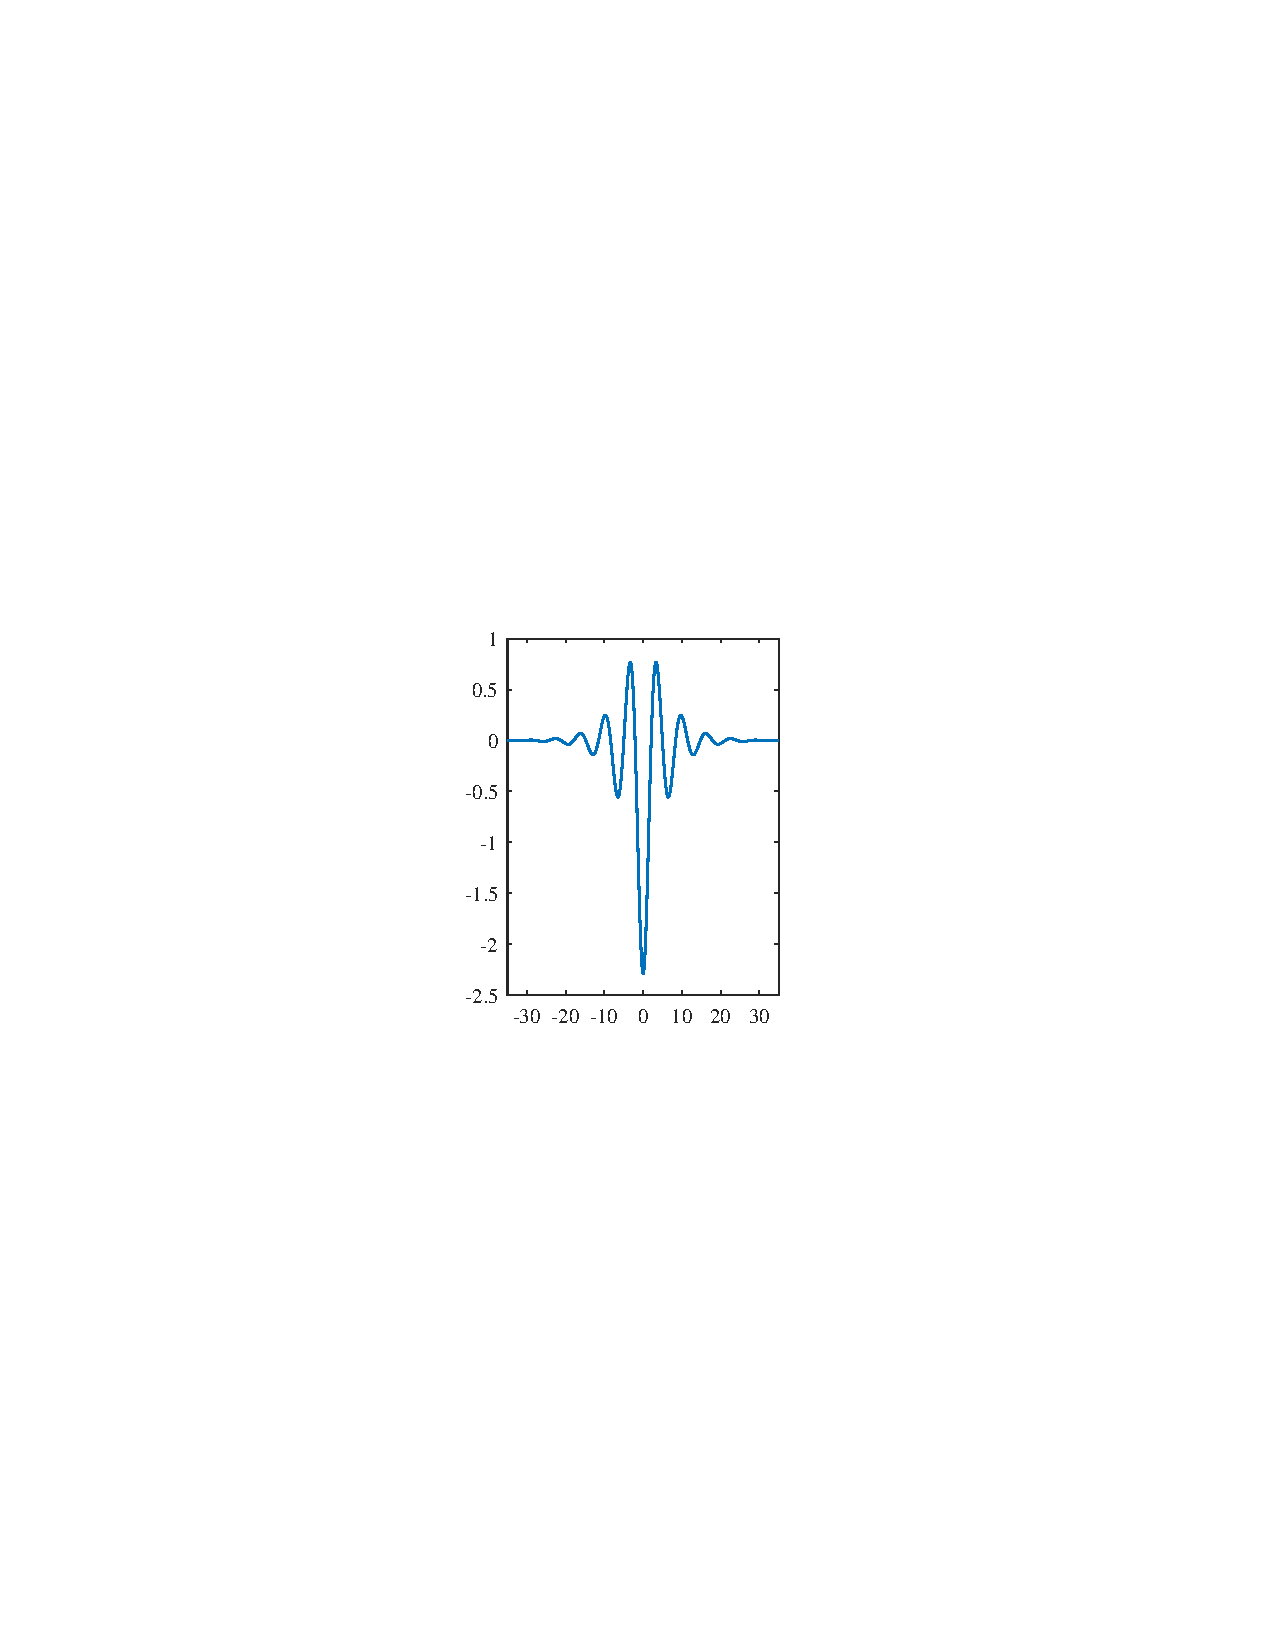
\includegraphics{images/chen/single1354}&
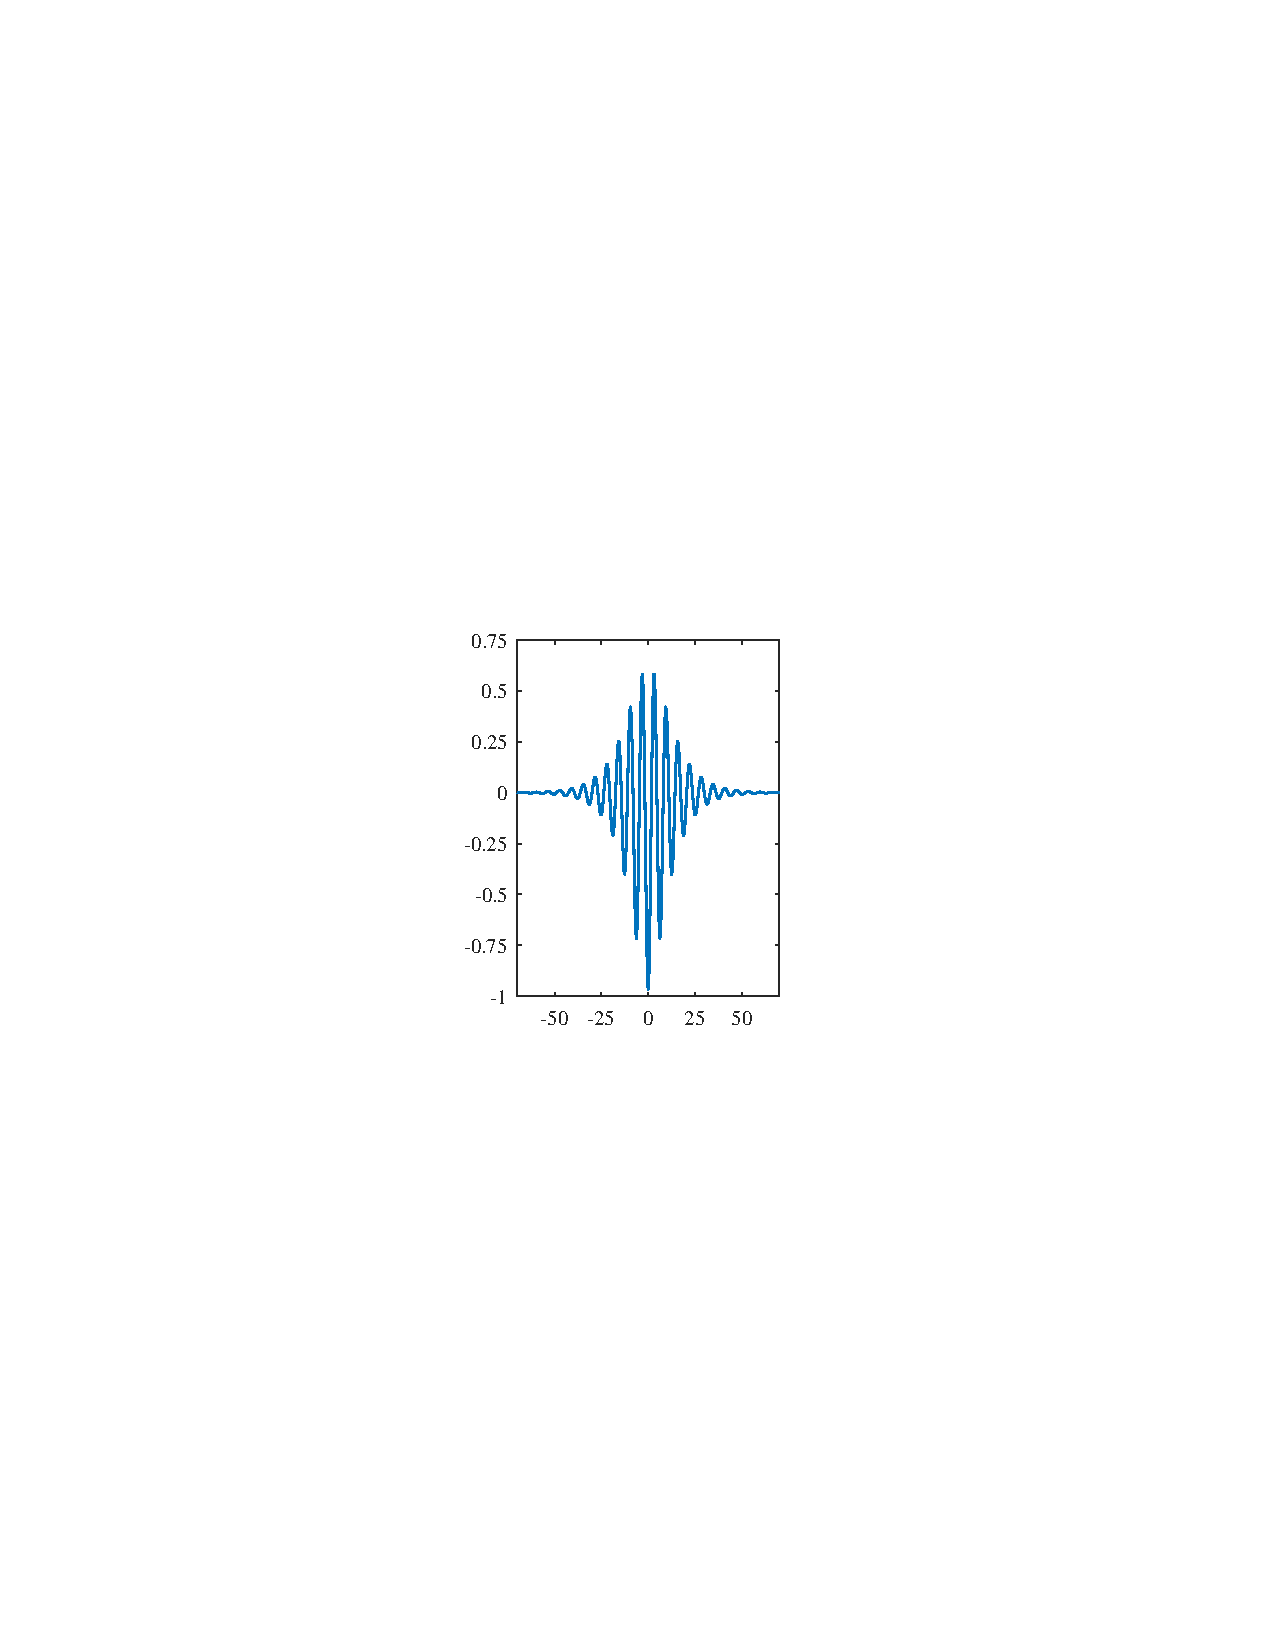
\includegraphics{images/chen/single14}
\end{tabular}
\includegraphics{images/chen/specA0}
\caption[Primary pulse solutions to Chen-McKenna]{Primary pulse solutions $U(x)$ to \cref{CheneqODE} for $c = 1.354$ (top left) and $c = 1.40$ (top right). In the bottom panel there is the spectrum of $\calA_0(U)$, the linearization of \cref{CheneqODE} about a single pulse $U(x)$ for $c = 1.3$. For the spectral plot we use finite difference methods with $N = 512$ and periodic boundary conditions. The left boundary of the essential spectrum is $\lambda\sim0.286$. The spectrum to the right of the boundary is discrete instead of continuous because of the boundary conditions. }
\label{fig:single1}
\end{figure}

%\begin{figure}[ht]
%\centering
%\includegraphics{specA0}
%\caption{Spectrum of $\calA_0(U)$, the linearization of \cref{CheneqODE} about a single pulse $U(x)$ for $c = 1.3$. We use finite difference methods with $N = 512$ and periodic boundary conditions.}
%\label{fig:specA0}
%\end{figure}

We can construct multi-pulse solutions numerically by joining together multiple copies of the primary pulse and using Matlab's \texttt{fsolve} function. Consecutive distances between peaks given by \cref{multiexist}. The first four double pulse solutions are shown in the top two panels of \cref{fig:double}. These double pulses are numbered using the integer $k_1$ from \cref{multiexist}. We verify \cref{multiexist}(b) numerically by computing the spectrum of $\calA_0(U_2)$. The spectrum of $\calA_0(U_2)$ for double pulses 0 and 1 are shown in the bottom two panels of \cref{fig:double}. In both cases, there is an eigenvalue at 0. For double pulse 0, there is an additional positive eigenvalue near 0, and for double pulse 1, there is an additional negative eigenvalue near 0.

\begin{figure}[ht]
\centering
\begin{tabular}{cc}
%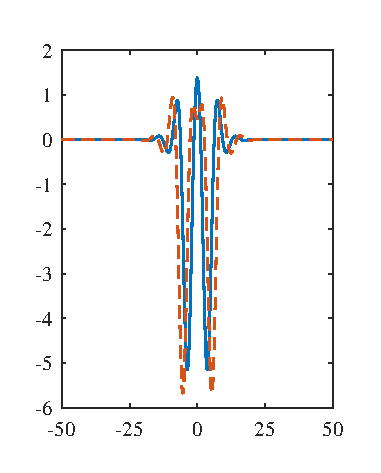
\includegraphics{double12_12}&
%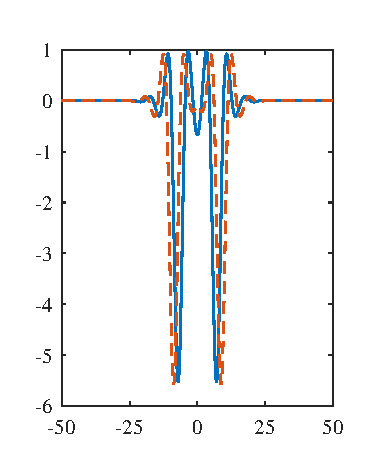
\includegraphics{double12_34}\\
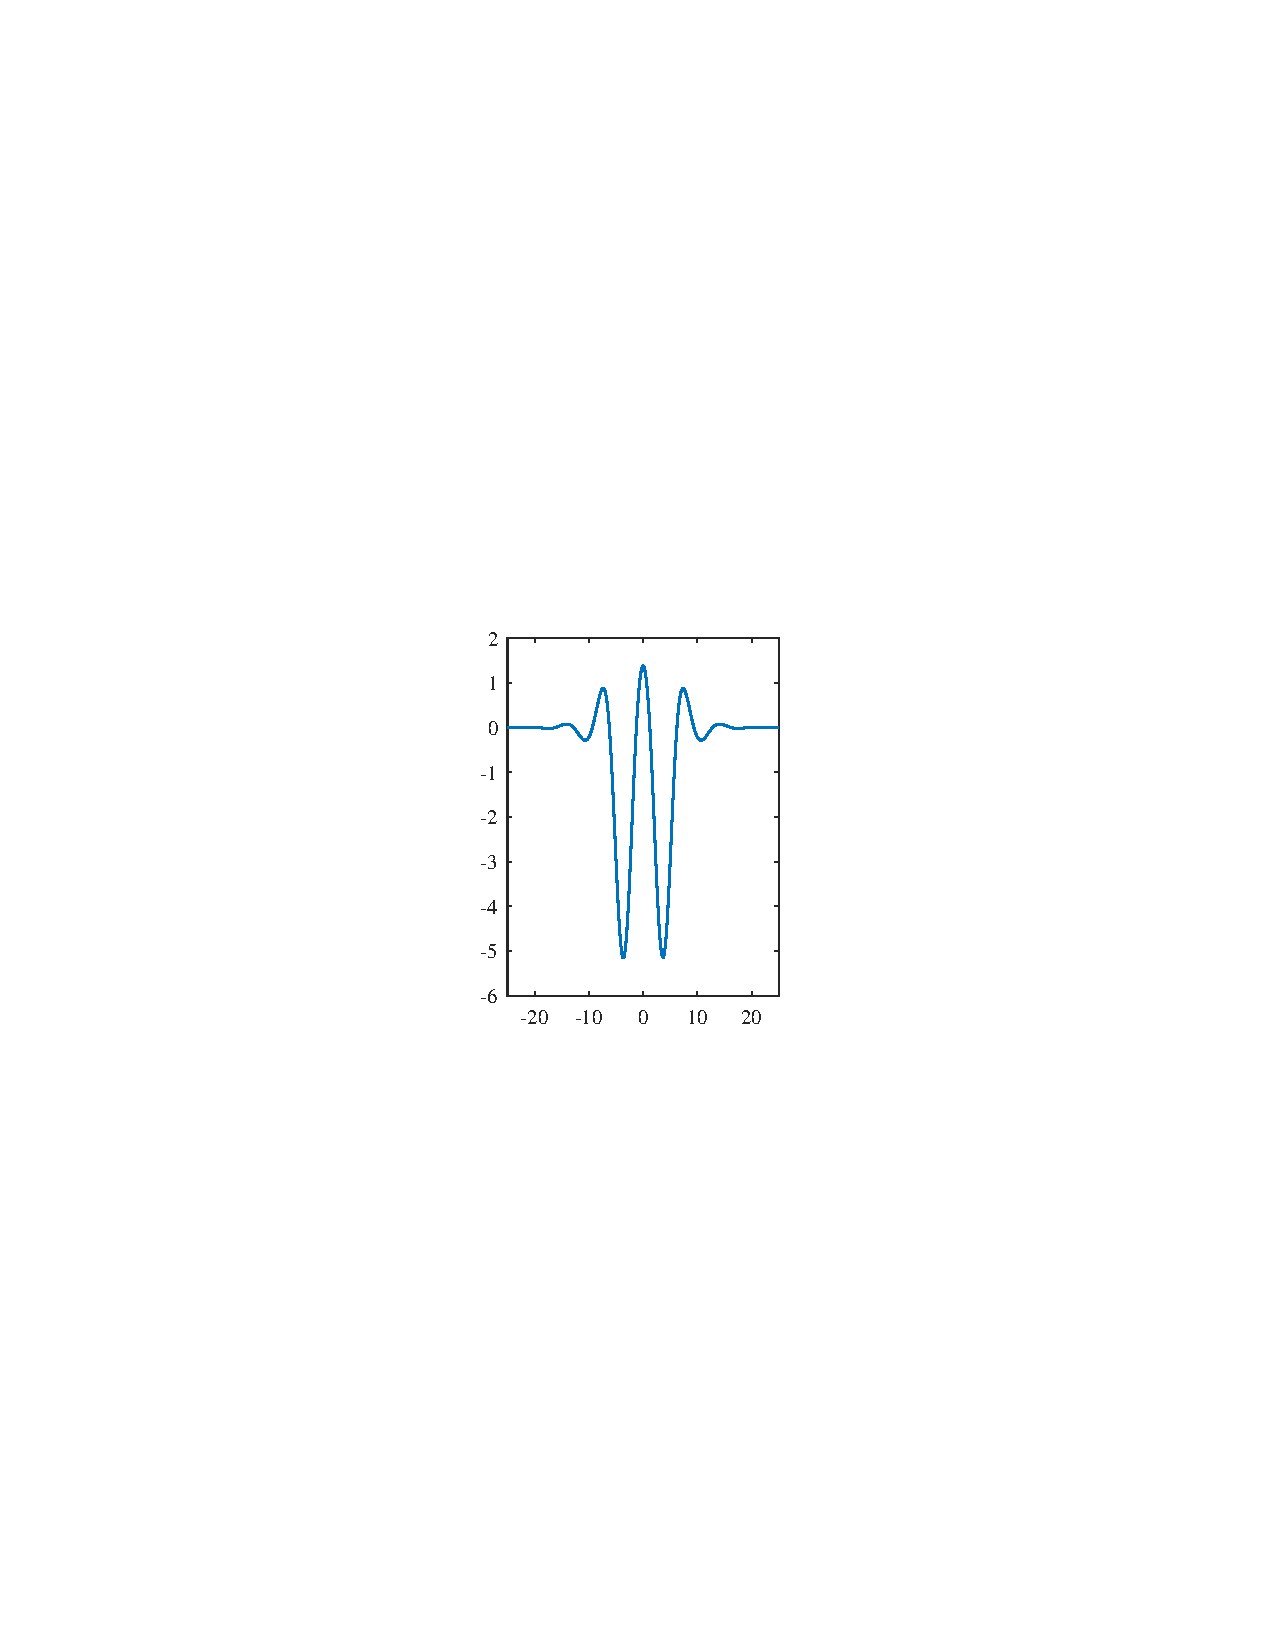
\includegraphics{images/chen/double1}&
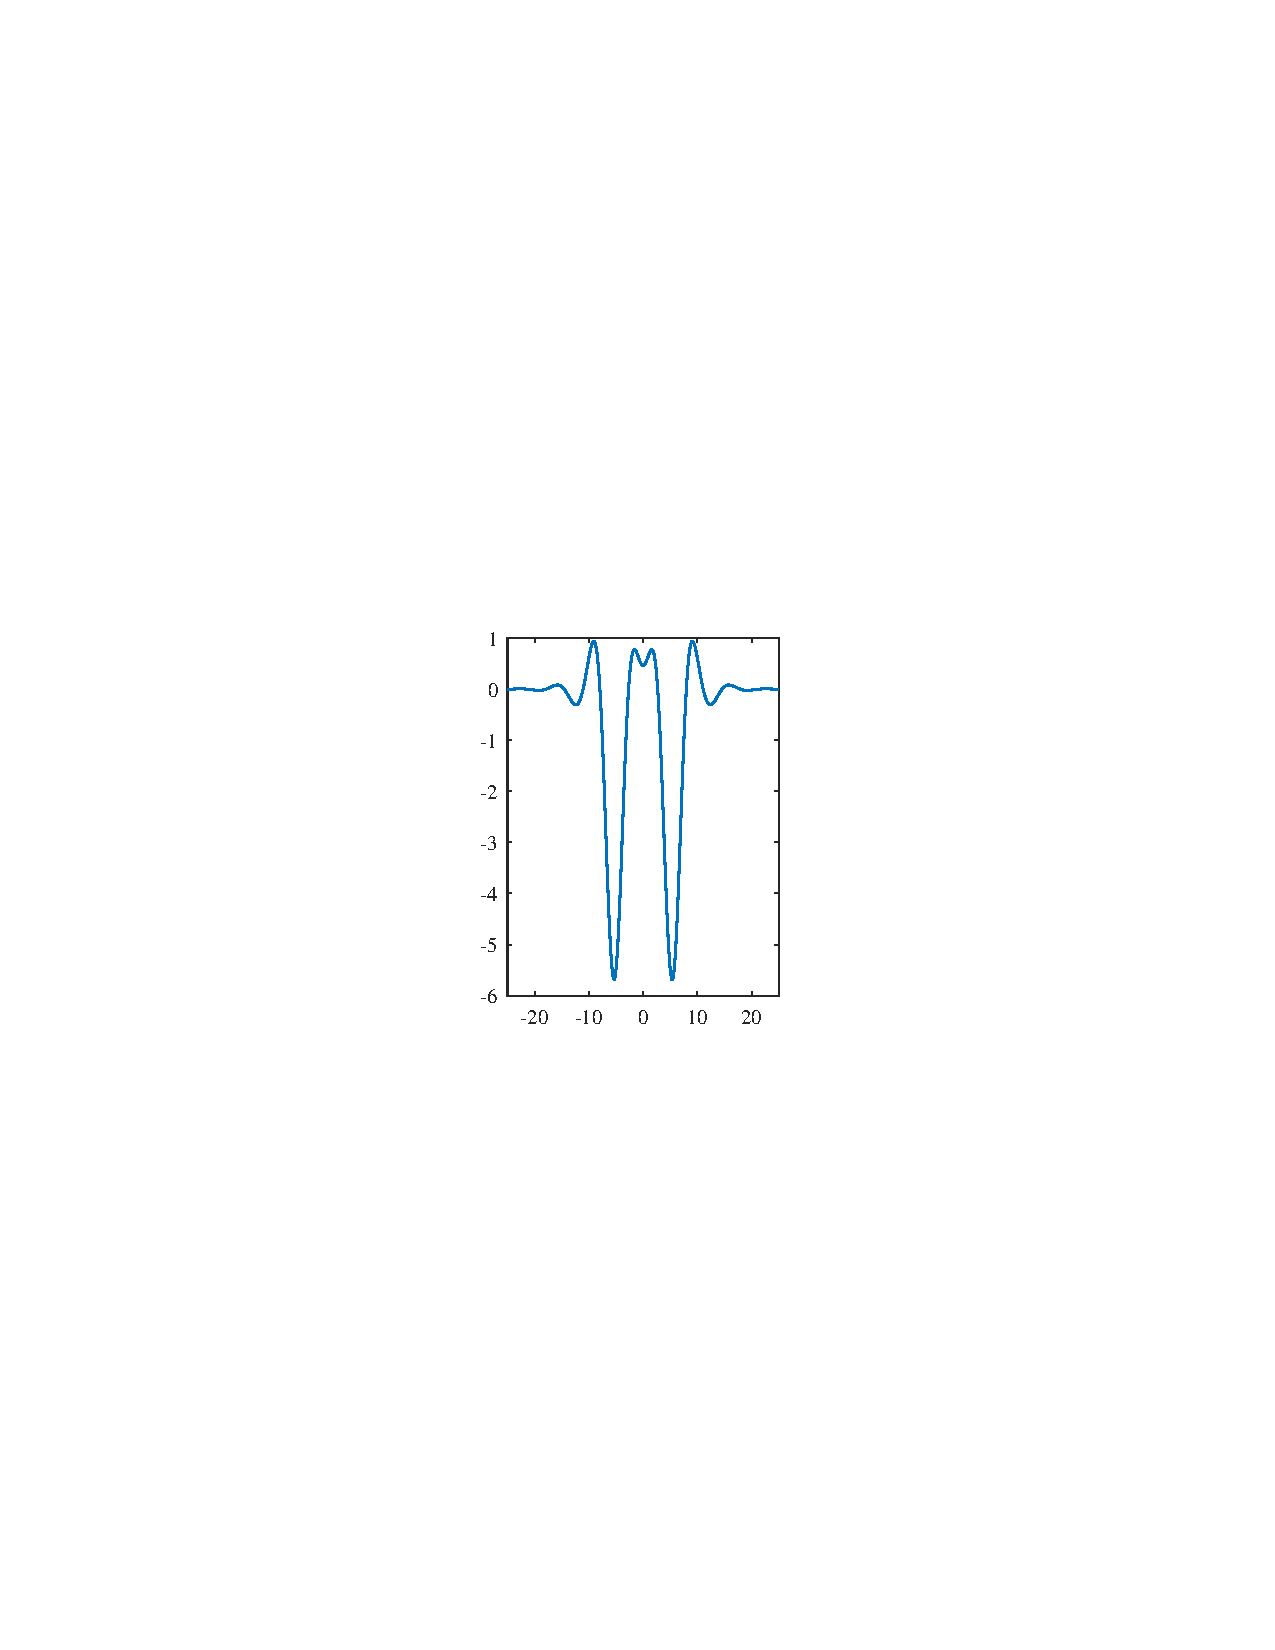
\includegraphics{images/chen/double2}\\
\includegraphics{images/chen/specA0d1.pdf}&
\includegraphics{images/chen/specA0d2.pdf}
\end{tabular}
\caption[Double pulse solutions to Chen-McKenna]{Double pulse solutions $U_2(x)$ to \cref{CheneqODE} for $c = 1.2$. The top left panel shows double pulse 0, and the top right panel shows double pulse 1. In the bottom two panels we see the associated spectrum for $\calA_0(U_2)$: double pulse 0 on the left, and double pulse 1 on the right.}
\label{fig:double}
\end{figure}

%\begin{figure}[ht]
%\centering
%\begin{tabular}{cc}
%\includegraphics{specA0d1}&
%\includegraphics{specA0d2}
%\end{tabular}
%\caption{Eigenvalues of $\calA_0(U_2)$ for $c = 1.2$. Double pulses 0 (left) and 1 (right).}
%\label{fig:specA0double}
%\end{figure}

We verify \cref{stabcrit} by computing the polynomial eigenvalues of \cref{quadeig} directly using the Matlab package \texttt{quadeig} from \cite{Hammarling2013}. For double pulse 0, $\calA_0(U_2)$ has one positive small magnitude eigenvalue; thus, by \cref{stabcrit}, equation \cref{quadeig} has a polynomial eigenvalue with positive real part. For double pulse 1, the small magnitude eigenvalue of $\calA_0(U_2)$ is negative; thus by \cref{stabcrit}, since the distance between the two peaks is sufficiently large, the polynomial eigenvalues of \cref{quadeig} are purely imaginary. These are shown in \cref{fig:quadeigdouble}.

\begin{figure}[ht]
\centering
\begin{tabular}{cc}
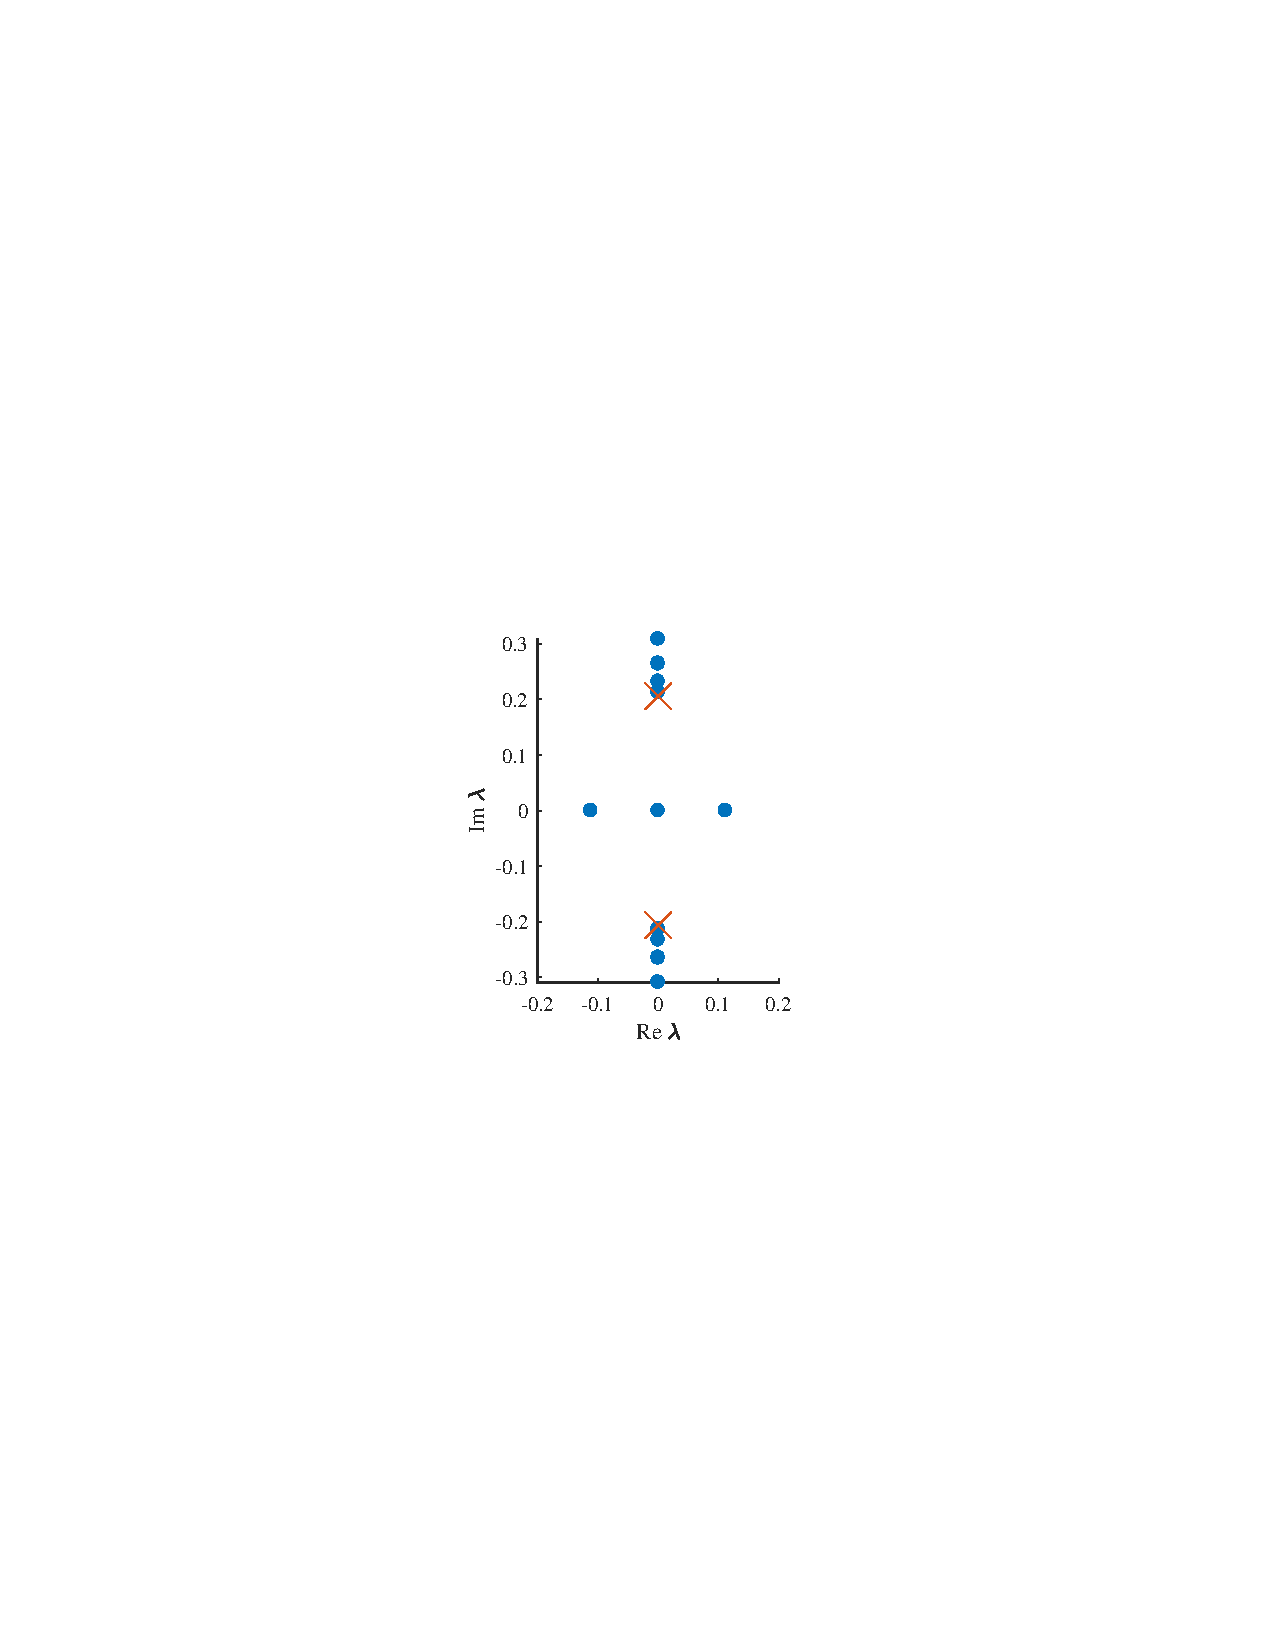
\includegraphics{images/chen/spec12_double1}&
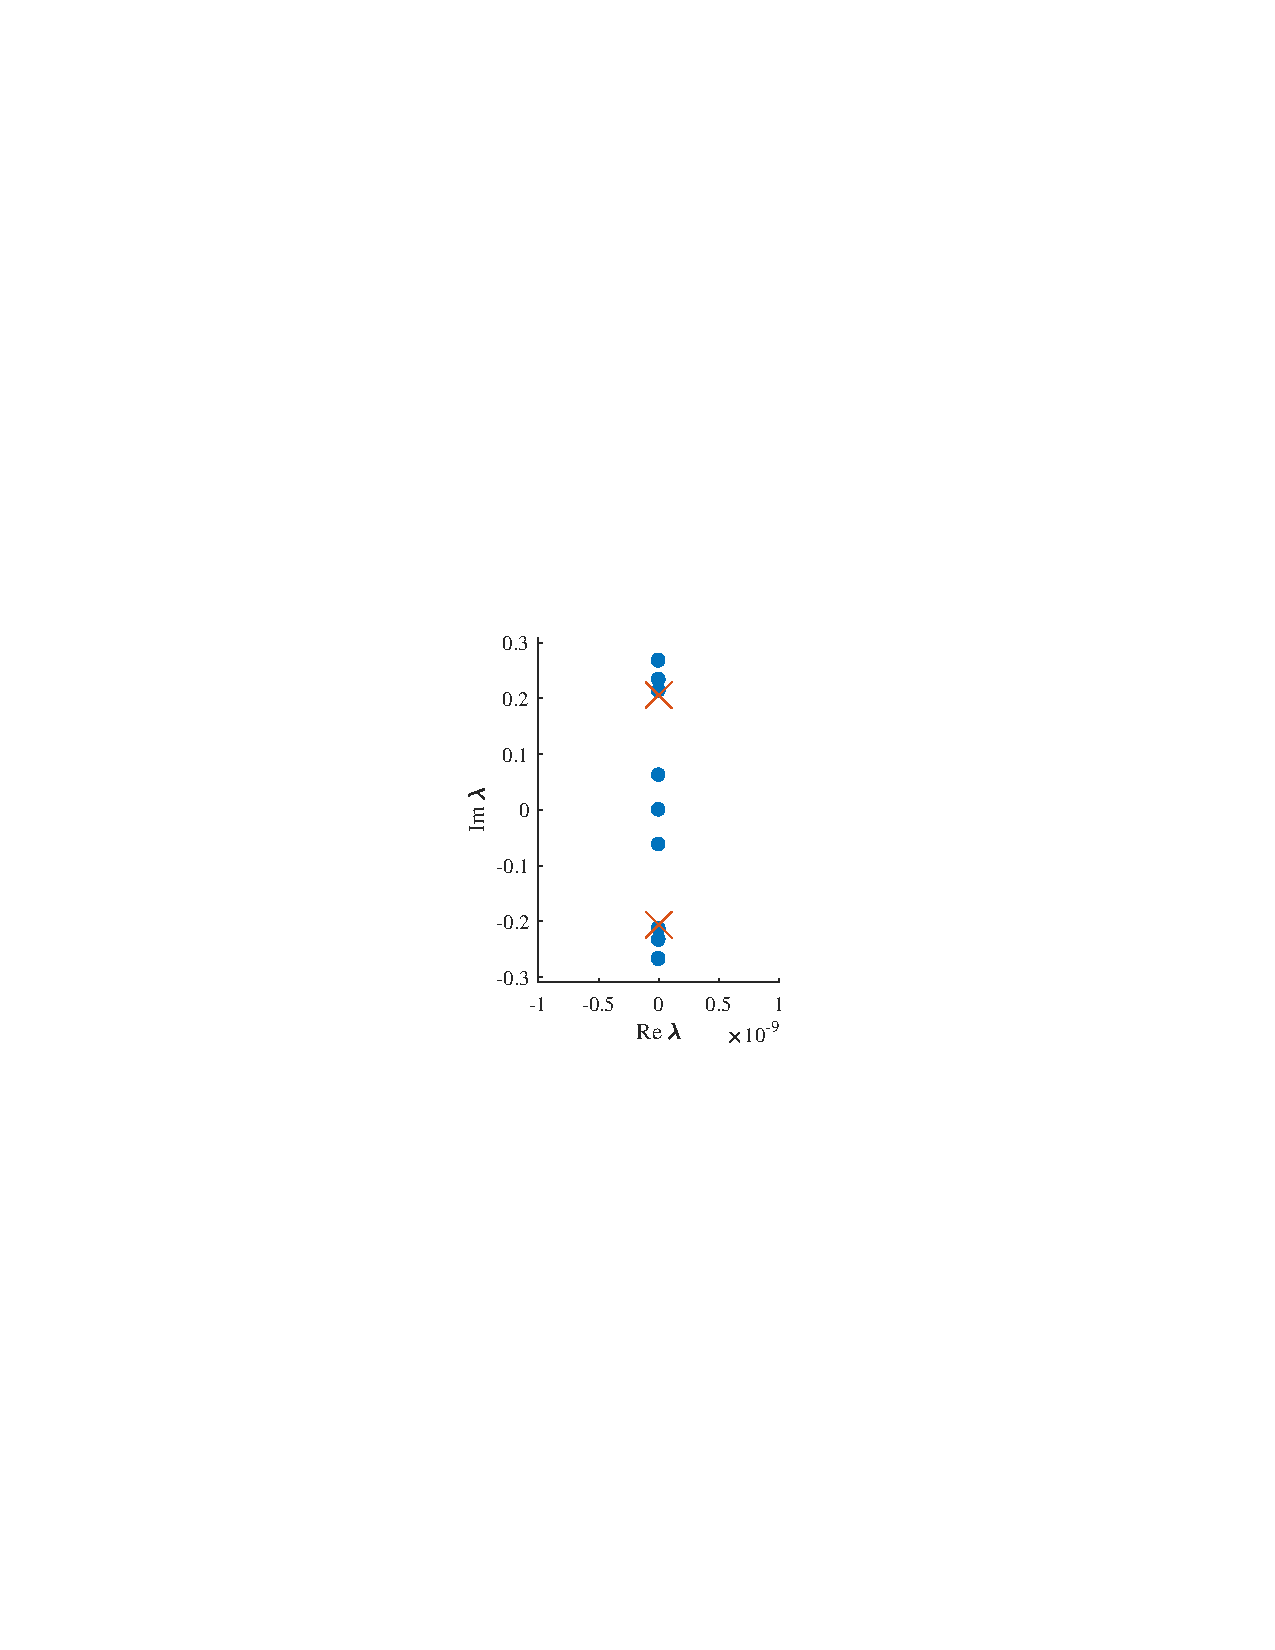
\includegraphics{images/chen/spec12_double2}
\end{tabular} 
\caption[Eigenvalues for double pulses in Chen-McKenna]{Polynomial eigenvalues of \cref{quadeig} for double pulses 0 (left) and 1 (right) for $c=1.2$. The eigenvalues are marked with a filled (blue) circle, and the edge of the essential spectrum is marked with a (red) cross. The essential spectrum is discrete instead of continuous because of the boundary conditions. For the right panel the two purely imaginary polynomial eigenvalues nearest the origin have negative Krein signature. Here we use finite difference methods with $N = 512$ and periodic boundary conditions.}
\label{fig:quadeigdouble}
\end{figure}

\section{Proof of \cref{Kreindiag}}\label{s:kreinproof}

Using \cref{multiexist}, let $U_n(x)$ be an $n-$modal solution to \cref{CheneqODE}, and let $\{\nu_1, \dots, \nu_n\}$ be the small magnitude eigenvalues of $\calA_0(U_n)$ with corresponding eigenfunctions $\{ s_1, \dots, s_n \}$. Since $\calA_0(U_n)$ is self-adjoint, the $s_i$ are orthogonal, and for the sake of convenience scale them so that,
\begin{equation}\label{orthoeigs}
\langle s_i, s_j \rangle = \|\partial_x U \|^2 \delta_{ij}.
\end{equation}
Typically, we assume these eigenfunctions also have unit length.  However, this is not important in the construction of the Krein matrix, nor in the derived properties.

By \cite[Lemma 5.6]{kapitula2019}, and using the normalization of \cref{orthoeigs}, for small $|z|$ the Krein matrix is the $n \times n$ matrix,
\begin{equation}\label{Kreinform}
-\frac{\vK_S(z)}{z} = \|\partial_xU_n\|^2 \text{diag}(\nu_1, \dots, \nu_n) + \overline{z}\vK_1
- \overline{z}^2 ( \|\partial_xU_n\|^2\vI_n - \vK_2) + \mathcal{O}(|z|^3),
\end{equation}
where
\begin{equation}\label{defK1}
(\vK_1)_{jk} = \langle s_j, \rmi\calA_1 s_k \rangle,
\end{equation}
and
\begin{equation}\label{defK2}
(\vK_2)_{jk} = \langle \calA_1 s_j, P_{S^\perp}(P_{S^\perp} \calA_0(U_n)P_{S^\perp})^{-1} P_{S^\perp}\calA_1 s_k \rangle .
\end{equation}
This is, to leading order, a matrix-valued quadratic polynomial in $z$ (and its complex conjugate). %If we take $z \in \R$, the Krein matrix is Hermitian.\\
We now prove \cref{Kreindiag} in a series of lemmas. In all that follows, $C$ refers to a constant independent of $x$, but it may have a different value each time it is used. The first lemma is a bound on the product of exponentially separated pulses.

\begin{lemma}\label{expseplemma}
Let $U_+(x)$ and $U_-(x)$ be localized pulses which decay exponentially with rate $\alpha$ and whose peaks are separated by a distance $2 X$. We have the following bounds,
\begin{equation}\label{expsepbound1}
\sup_{x \in \R} | U_-(x) U_+(x)|\leq C \rme^{-2 \alpha X},
\end{equation}
and
\begin{equation}\label{expsepbound2}
|\langle U_-(x) U_+(x) \rangle |\leq C \rme^{-(3 \alpha/2) X}.
\end{equation}
\begin{proof}
Without loss of generality, let $U_\pm(x)$ be exponentially localized peaks centered at $\pm X$, thus $|U_-(x)| \leq C e^{-\alpha|x + X|}$ and $|U_+(x)| \leq C \rme^{-\alpha|x - X|}$. For $x \in (-\infty, -X]$,
\begin{align}\label{endprodbound}
| U_-(x) U_+(x) | &\leq C \rme^{\alpha(x + X)} \rme^{\alpha(x - X)} = C \rme^{2 \alpha x} \leq C \rme^{-2 \alpha X}
\end{align}
and for $x \in [-X, 0]$,
\begin{align}\label{middleprodbound}
| U_-(x) U_+(x) | &\leq C \rme^{-\alpha(x + X)} \rme^{\alpha(x - X)} = C \rme^{-2 \alpha X}
\end{align}
Bounds on $[0, X]$ and $[X, \infty)$ are similar. Since these are independent of $x$, we obtain the bound \cref{expsepbound1}.

For the bound \cref{expsepbound2}, we split the integral into four pieces.
\begin{equation}
\begin{aligned}
| \langle U_-(x), &U_+(x) \rangle |
\leq \int_{-\infty}^{-X} |U_-(x) U_+(x)| \rmd x + \int_{-X}^0 |U_-(x) U_+(x)|\rmd x \\
&+\int_0^X |U_-(x) U_+(x)| \rmd x +\int_X^\infty |U_-(x) U_+(x)| \rmd x
\end{aligned}
\end{equation}
For the first integral, we use \cref{endprodbound} to get
\begin{align*}
\int_{-\infty}^{-X} |q_-(x) q_+(x)| \rmd x &\leq C \int_{-\infty}^{-X} \rme^{2 \alpha x} \rmd x = C \rme^{-2 \alpha X}
\end{align*}
For the second integral, we use \cref{middleprodbound} to get
\begin{align*}
\int_{-X}^0 |q_-(x) q_+(x)| \rmd x &\leq C \int_{-X}^0 \rme^{-\alpha(x + X)} \rme^{\alpha(x - X)} \rmd x \leq C \int_{-X}^0 \rme^{-\alpha(x + X)/2}\rme^{\alpha(x - X)} \rmd x \\
&\leq C \rme^{-(3 \alpha/2) X } \int_{-X}^0 \rme^{(\alpha/2)x} \rmd x \leq C \rme^{-(3 \alpha/2) X }
\end{align*}
The third and fourth integrals are similar. Combining these, we obtain \cref{expsepbound2}.
\end{proof}
\end{lemma}

\begin{remark}
If the hypotheses of \cref{expseplemma} are satisfied, we say that $U_+(x)$ and $U_-(x)$ are exponentially separated by $2X$.
\end{remark}

Next, we obtain a bound on the matrix $\vK_1$.
% lemma : K1 is small
\begin{lemma}\label{K1small}
For the matrix $\vK_1$ in \cref{Kreinform},
\begin{equation}\label{K1final}
\vK_1 = \mathcal{O}(\rme^{-(3 \alpha/2) X_{\mathrm{min}}}).
\end{equation}
\end{lemma}

\begin{proof}
Substituting $\calA_1 = -2c\partial_x$ into \cref{defK1}, $(\vK_1)_{jk} = \rmi 2 c \langle s_j, \partial_xs_k \rangle$. Using the expansion \cref{sj} from Theorem \ref{multiexist},
\begin{equation}\label{K1exp}
\begin{aligned}
\langle s_j ,\partial_xs_k \rangle
&= \sum_{m = 1}^{n} d_{jm} d_{km} \langle \partial_xU^m_x, \partial_x^2U^m \rangle
+ \sum_{m \neq\ell} d_{jm} d_{k\ell} \langle \partial_xU^m, \partial_x^2U^\ell \rangle\\
&\qquad
+ \langle s_j, \partial_x w_k \rangle
+ \sum_{\ell = 1}^{n} d_{k\ell} \langle w_j, \partial_x^2U^\ell \rangle.
\end{aligned}
\end{equation}
By translation invariance of the inner product on $L^2(\R)$,
\[
\langle \partial_xU^m, \partial_x^2U^m \rangle = \langle \partial_xU, \partial_x(\partial_xU) \rangle = 0,
\]
since the operator $\partial_x$ is skew-symmetric. For $m \neq\ell$, $U^m$ and $U^\ell$ are exponentially separated by at least $2 X_{\mathrm{min}}$; thus, by Lemma \ref{expseplemma},
\[
\langle \partial_xU^m, \partial_x^2U^\ell \rangle = \mathcal{O}(\rme^{-(3 \alpha/2) X_{\mathrm{min}}}).
\]
The last two terms in \cref{K1exp} are $\mathcal{O}(\rme^{-2 \alpha X_{\mathrm{min}}})$ using H\"{o}lder's inequality and the bound \cref{sjwbound} from \cref{multiexist}, which applies to $\partial_x w_k$ as well as $w_j$. Combining these estimates we obtain \cref{K1final}.
\end{proof}

Using the expansion \cref{sj} from \cref{multiexist}, the matrix $\vK_2$ in \cref{Kreinform} becomes,
\begin{equation}\label{K2expansion}
\begin{aligned}
&(\vK_2)_{jk}
= 4 c^2 \left\langle\sum_{m = 1}^{n} d_{jm} \partial_x^2U^m + \partial_x w_j,\right. \\
&\qquad\left.\sum_{\ell = 1}^{n} d_{k\ell} P_{S^\perp} (P_{S^\perp} \calA_0(U_n)P_{S^\perp})^{-1} P_{S^\perp} \partial_x^2U^\ell + P_{S^\perp} (P_{S^\perp} \calA_0(U_n)P_{S^\perp})^{-1} P_{S^\perp}\partial_xw_k \right\rangle.
\end{aligned}
\end{equation}
Before we can evaluate this expression, we need to look at $(P_{S^\perp} \calA_0(U_n)P_{S^\perp})^{-1}$.

% lemma : P_{S^\perp} \calA_0(U_n) |_{S^\perp} invertible

\begin{lemma}\label{PA0inv}
$P_{S^\perp} \calA_0(U_n) P_{S^\perp}: S^\perp \rightarrow S^\perp$ is an invertible linear operator with bounded inverse.
\end{lemma}

\begin{proof}
By \cref{A0ess}, the essential spectrum of $\calA_0(U_n)$ is bounded away from 0, thus the operator $\calA_0(U_n)$ is Fredholm with index 0. Since $\calA_0(U_n)$ is self-adjoint, $P_{S^\perp} \calA_0(U_n)$ is also self-adjoint, and it is not hard to show that $P_{S^\perp} \calA_0(U_n)$ is Fredholm with index 0 and has kernel $S$. Thus the restriction $P_{S^\perp} \calA_0(U_n)|_{S^\perp} = P_{S^\perp} \calA_0(U_n) P_{S^\perp}$ is invertible on $S^\perp$. By the definition of $S$ and \cref{multiexist}, $P_{S^\perp}\calA_0(U_n)P_{S^\perp}$ has no eigenvalues of magnitude less than $\delta$. Since the essential spectrum of $\calA_0(U_n)$ is bounded away from 0, by the resolvent bound for normal operators, the linear operator $(P_{S^\perp} \calA_0(U_n)P_{S^\perp})^{-1}$ is bounded on $S^\perp$.
\end{proof}

Before we can evaluate the term $(P_{S^\perp} \calA_0(U_n)P_{S^\perp})^{-1} P_{S^\perp}\partial_x^2U^\ell$ from \cref{K2expansion}, we will need the following lemma which gives an expansion for $e^{U_n(x)}$.

% lemma : separation of exponential e^{U_n(x)}

\begin{lemma}\label{expsep}
For the $n-$pulse, $U_n(x)$, and for all $i = 1, \dots, n$,
\[%begin{equation}\label{expUnexpansion}
\exp(U_n(x)) = \exp( U^i(x)) + \sum_{j \neq i} (\exp(U^j(x)) - 1) + \mathcal{O}(\rme^{-\alpha X_{\mathrm{min}}})
\]%end{equation}
\end{lemma}

\begin{proof}
Fix $i$ in the expansion \eqref{qn} and let $S(x) = \sum_{j \neq i} U_j(x)$, so that $U_n = U^i + S + \mathcal{O}(e^{-\alpha X_{\mathrm{min}}})$. Since $U_n(x)$ is bounded,
\[
\begin{aligned}
\exp(U_n(x)) &= \exp( U^i(x) )\exp(S(x))(1 + \mathcal{O}(\rme^{-\alpha X_{\mathrm{min}}})) \\
&= \exp( U^i(x) )\exp(S(x)) + \mathcal{O}(\rme^{-\alpha X_{\mathrm{min}}}).
\end{aligned}
\]
Using the Taylor expansion for the exponential,
\[
\begin{aligned}
\exp( U^i(x) )\exp(S(x))
&= \sum_{m=0}^\infty \frac{U^i(x)^m}{m!}
\sum_{n=0}^\infty \frac{S(x)^n}{n!} \\
&= \sum_{m=0}^\infty \frac{U^i(x)^m}{m!}
+ \sum_{n=0}^\infty\frac{S(x)^n}{n!} - 1 +
\sum_{m=1}^\infty \frac{U^i(x)^m}{m!}
\sum_{n=1}^\infty \frac{S(x)^n}{n!} \\
&= \exp(U^i(x)) + \exp(S(x)) - 1 +
\sum_{m=1}^\infty \frac{U^i(x)^m}{m!}
\sum_{n=1}^\infty \frac{S(x)^n}{n!}
\end{aligned}
\]
For the last term on the RHS,
\[
\begin{aligned}
\left| \sum_{m=1}^\infty \frac{U^i(x)^m}{m!} \sum_{n=1}^\infty \frac{S(x)^n}{n!} \right|
&= \left| U^i(x)S(x)\right| \sum_{m=0}^\infty \frac{|U^i(x)|^m}{(m+1)!} \sum_{n=0}^\infty \frac{|S(x)|^n}{(n+1)!} \\
&\leq \left| U^i(x)S(x) \right| e^{|U^i(x)|}e^{|S(x)|} \\
&\leq C \rme^{-2 \alpha X_{\mathrm{min}}},
\end{aligned}
\]
where in the last line we used the fact that $U_n(x)$ is bounded together with the bound \cref{expsepbound1} from \cref{expseplemma}, since $U^i$ and each peak in $S$ are exponentially separated. Combining all of this,
\[
\begin{aligned}
\exp(U_n(x)) &= \exp(U^i(x)) + \exp(S(x)) - 1 + \mathcal{O}(\rme^{-\alpha X_{\mathrm{min}}})
\end{aligned}
\]
Repeat this procedure $n - 2$ more times to get the result.
\end{proof}

We can now evaluate $(P_{S^\perp} \calA_0(U_n) P_{S^\perp})^{-1} P_{S^\perp}\partial_x^2U^\ell$.

% lemma : evaluation of (P_{S^\perp} \calA_0(U_n)|_{S^\perp})^{-1} P_{S^\perp} q^i_{xx}

\begin{lemma}\label{PA0invqxx}
\begin{equation}\label{invqxx}
(P_{S^\perp} \calA_0(U_n)P_{S^\perp})^{-1} P_{S^\perp}\partial_x^2U^\ell = -\frac{1}{2c}P_{S^\perp}\partial_cU^\ell
+ \mathcal{O}(\rme^{-2 \alpha X_{\mathrm{min}}}).
\end{equation}
\end{lemma}

\begin{proof}
Let $y = (P_{S^\perp} \calA_0(U_n)P_{S^\perp})^{-1} P_{S^\perp}\partial_x^2U^\ell$, which is well-defined by Lemma \ref{PA0inv}. Since $P_{S^\perp}\partial_x^2U^\ell$ is smooth and $(P_{S^\perp} \calA_0(U_n)P_{S^\perp})^{-1}$ is bounded, $y$ is smooth as well and is the unique solution to the equation
\begin{equation}\label{Linstart}
(P_{S^\perp} \calA_0(U_n) P_{S^\perp})y = P_{S^\perp}\partial_x^2U^\ell.
\end{equation}
Using Lin's method as in \cite{Sandstede1998}, we will look for a solution to \cref{Linstart} of the form,
\begin{equation}\label{Linsolform}
\tilde{y} = -\frac{1}{2c} P_{S^\perp}\partial_cU^\ell + \tilde{w}.
\end{equation}
This ansatz is suggested by
\begin{equation}\label{uc}
\calA_0(U) \partial_c U = -2 c\partial_x^2 U,
\end{equation}
which we obtain by taking $u = U$ in equation \cref{CheneqODE} and differentiating with respect to $c$, which we can do since $U$ is smooth in $c$ by \cref{Uexistshyp}. Substituting \cref{Linsolform} into \cref{Linstart} and simplifying, we obtain the equation for $\tilde{w}$
\begin{equation}\label{A0heq}
\calA_0(U_n)\tilde{w} + h(x) = 0,
\end{equation}
where $h(x)$ is a small remainder term with uniform bound $\|h(x)\|_\infty = \mathcal{O}(\rme^{-\alpha X_{\mathrm{min}}})$. Using \cref{expsep}, for $j = 1, \dots, n$ we can write the operator $\calA_0(U_n)$ as,
\begin{equation}\label{A0expansion}
\calA_0(U_n) = \calA_0(U^j) + \sum_{k \neq j} (\rme^{U^k(x)} - 1) + \tilde{h}(x),
\end{equation}
where $\tilde{h}(x)$ is another small remainder term with uniform bound $\|\tilde{h}\|_\infty = \mathcal{O}(\rme^{-\alpha X_{\mathrm{min}}})$.

We now follow the procedure in \cite{Sandstede1998}, which we briefly outline below. Let $W = (\tilde{w}, \partial_x\tilde{w},\partial_x^2 \tilde{w},\partial_x^3 \tilde{w})$. As in \cite{Sandstede1998}, we rewrite \cref{A0heq} as a first-order system for $W$, and we take $W$ to be a piecewise function consisting of the $2n$ pieces $W_j^\pm, j = 1, \dots, n$, where
\begin{align*}
W_j^-(x) &\in C^0([-X_{j-1}, 0]) \\
W_j^+(x) &\in C^0([0, X_j])
\end{align*}
with $X_0 = X_n = \infty$. Following this procedure, and using the expansions \cref{A0expansion} for $\calA_0(U_n)$ on the $j$-th piece, we obtain the system of equations
\begin{equation}\label{Wsystem}
\begin{aligned}
(W_j^\pm)'(x) = A(U(x)) W_j^\pm(x) &+ G_j(x) W_j^\pm(x)+ B H(x) \\
W_j^+(X_i) - W_{j+1}^-(-X_j) &= 0  \\
W_j^-(0) - W_j^+(0) &= 0
\end{aligned}
\end{equation}
where
\[
A(U(x)) = \begin{pmatrix}
0 & 1 & 0 & 0 \\
0 & 0 & 1 & 0 \\
0 & 0 & 0 & 1 \\
-e^{U(x)} & 0 & -c^2 & 0
\end{pmatrix},\quad
B = \begin{pmatrix}
0 & 0 & 0 & 0 \\
0 & 0 & 0 & 0 \\
0 & 0 & 0 & 0 \\
1 & 0 & 0 & 0
\end{pmatrix},
\]
and
\[
G_j(x) = \begin{pmatrix}
0 & 0 & 0 & 0 \\
0 & 0 & 0 & 0 \\
0 & 0 & 0 & 0 \\
\sum_{k \neq j} (1 - e^{U(x - \rho_{kj})}) & 0 & 0 & 0
\end{pmatrix},
\]
$\rho_{kj}$ is the signed distance from peak of $U^k$ to peak of $U^j$ in $U_n$, and $\|H\| = \mathcal{O}(\rme^{-\alpha X_{\mathrm{min}}})$. For $k \neq j$, $|\rho_{kj}| \geq 2 X_{\mathrm{min}}$. This implies $e^{U(x - \rho_{kj})} = \mathcal{O}(\rme^{-\alpha X_{\mathrm{min}}})$ on the $j$-th piece, thus we can use a Taylor expansion to show $\|G_j\| = \mathcal{O}(\rme^{-\alpha X_{\mathrm{min}}})$. Following the procedure in \cite{Sandstede1998}, we obtain a unique piecewise solution $W_j^\pm$ to the first two equations of \cref{Wsystem}. The third equation is generally not satisfied, so what we have constructed is a unique solution $\tilde{y}$ of the form \cref{Linsolform} to \cref{Linstart} which is continuous except for $n - 1$ jumps. By uniqueness, we must have $\tilde{y} = y$, thus $y$ is actually of the form \cref{Linsolform} with $\tilde{w}$ smooth. Finally, Lin's method gives us the uniform bound
$\|\tilde{w}\|_\infty = \mathcal{O}(\rme^{-2 \alpha X_{\mathrm{min}}})$, from which \cref{invqxx} follows.
\end{proof}

We prove one more lemma before we evaluate the matrix $\vK_2$ from \cref{Kreinform}.

% lemma : orthogonality of coefficients d_{jk}

\begin{lemma}\label{orthogonald}
For the coefficients $d_{jk}$ in \cref{sj} from \cref{multiexist},
\begin{equation}\label{dsum}
\sum_{m = 1}^{n} d_{jm} d_{km} = \delta_{jk} + \mathcal{O}(\rme^{-(3 \alpha/2) X_{\mathrm{min}}}).
\end{equation}
\end{lemma}

\begin{proof}
% I fixed stuff here, 12/27
Using the expansion \cref{sj} from \cref{multiexist},
\[
\begin{aligned}
\langle s_j, s_k \rangle
&= \sum_{m = 1}^{n} d_{jm} d_{km} \langle \partial_xU^m,\partial_xU^m \rangle
+ \sum_{m \neq \ell} d_{jm} d_{k\ell} \langle \partial_xU^m, \partial_xU^\ell \rangle\\
&\qquad
+ \langle s_j, w_k \rangle
+ \sum_{\ell = 1}^{n} d_{k\ell} \langle w_j, \partial_xU^\ell \rangle.
\end{aligned}
\]
As in \cref{K1small}, the second term on the RHS is $\mathcal{O}(\rme^{-(3 \alpha/2) X_{\mathrm{min}}})$, and the last two terms on the RHS are $\mathcal{O}(\rme^{-2 \alpha X_{\mathrm{min}}})$. By translation invariance, $\langle \partial_xU^m, \partial_xU^m \rangle = \langle \partial_xU, \partial_xU \rangle = \|\partial_xU\|^2$ for all $m$. This reduces to
\[
\langle s_j, s_k \rangle
= \|\partial_xU\|^2 \sum_{m = 1}^{n} d_{jm} d_{km} + \mathcal{O}(\rme^{-(3 \alpha/2) X_{\mathrm{min}}}).
\]
Dividing by $\|\partial_xU\|^2$ and using the orthogonality relation \cref{orthoeigs} gives us \cref{dsum}.
\end{proof}

Finally, we can evaluate the matrix $\vK_2$ from \cref{Kreinform}.

% lemma : K2 approx diagonal

\begin{lemma}\label{K2diag}
For the matrix $\vK_2$ in \cref{Kreinform},
\begin{equation}\label{K2final}
(\vK_2)_{jk}
= -2 c\langle\partial_x^2 U, \partial_c U \rangle \delta_{jk} + \mathcal{O}(\rme^{-(3 \alpha/2) X_{\mathrm{min}}}).
\end{equation}
\end{lemma}

\begin{proof}
By \cref{PA0inv}, $(P_{S^\perp} \calA_0(U_n)P_{S^\perp})^{-1}$ is a bounded linear operator. Using the bound \cref{sjwbound} from \cref{multiexist},
\[
P_{S^\perp} (P_{S^\perp} \calA_0(U_n)|_{S^\perp})^{-1} P_{S^\perp}\partial_xw_k = \mathcal{O}(\rme^{-2 \alpha X_{\mathrm{min}}}).
\]
Using this and \cref{invqxx} from \cref{PA0invqxx}, \cref{K2expansion} becomes,
\[
\begin{aligned}
(\vK_2)_{jk}
&= 4 c^2 \left\langle \sum_{m = 1}^{n} d_{jm}\partial_x^2U^m + \partial_xw_j,
-\frac{1}{2c}\sum_{\ell = 1}^{n} d_{k\ell} P_{S^\perp}\partial_cU^\ell + \mathcal{O}(\rme^{-2 \alpha X_{\mathrm{min}}}) \right\rangle \\
&= -2 c \left( \sum_{m = 1}^{n} d_{jm} d_{km} \langle \partial_x^2U^m, P_{S^\perp} \partial_cU^m \rangle
+ \sum_{m\neq \ell} d_{jm} d_{k\ell} \langle \partial_x^2U^m, P_{S^\perp} \partial_cU^l \rangle\right.\\
&\qquad\qquad\left.+ \sum_{\ell=1}^n \langle \partial_xw_j, d_{k\ell}\partial_cU^\ell \rangle \right)
 + \mathcal{O}(\rme^{-2 \alpha X_{\mathrm{min}}}).
\end{aligned}
\]
For $m\neq\ell$, $\partial_x^2U^m$ and $\partial_cU^\ell$ are exponentially separated, thus the second term on the RHS is $\mathcal{O}(\rme^{-(3 \alpha/2) X_{\mathrm{min}}})$ by \cref{expseplemma}. Using H\"{o}lder's inequality and the remainder bound \cref{sjwbound}, the third term on the RHS is $\mathcal{O}(\rme^{-2 \alpha X_{\mathrm{min}}})$. Thus we are left with
\begin{equation}\label{K2step1}
\begin{aligned}
(\vK_2)_{jk}
&= -2 c \sum_{m = 1}^{n} d_{jm} d_{km} \langle \partial_x^2U^m, P_{S^\perp} \partial_cU^m \rangle + \mathcal{O}(\rme^{-(3 \alpha/2) X_{\mathrm{min}}}).
\end{aligned}
\end{equation}
To evaluate the inner product, we first evaluate $P_S \partial_c U^m$. Recalling the normalization \cref{orthoeigs} and using the expansion \cref{sj}, since the $s_j$ are orthogonal,
\[
\begin{aligned}
P_S &\partial_c U^m = \frac{1}{\|\partial_x U\|} \sum_{j=1}^n \langle s_j, \partial_c U^m \rangle \\
&= \frac{1}{\|\partial_x U\|} \sum_{j=1}^n \sum_{k=1}^n \langle d_{jk} \partial_x U^k + w_k, \partial_c U^m \rangle \\
&= \frac{1}{\|\partial_x U\|} \left( \sum_{j=1}^n d_{jm} \langle \partial_x U^m, \partial_c U^m \rangle + \sum_{j=1}^n \sum_{k \neq m}^n d_{jk} \langle \partial_x U^k, \partial_c U^m \rangle \right) + \mathcal{O}(\rme^{-2 X_{\mathrm{min}}}) \\
&= \frac{1}{\|\partial_x U\|} \sum_{j=1}^n d_{jm} \langle \partial_x U, \partial_c U \rangle + \mathcal{O}(\rme^{-(3 \alpha/2) X_{\mathrm{min}}}) \\
&= \mathcal{O}(\rme^{-(3 \alpha/2) X_{\mathrm{min}}}).
\end{aligned}
\]
The third line follows from \cref{expseplemma} since $\partial_x U^k$ and $\partial_c U^m$ are exponentially separated for $k \neq m$, and in the fourth line we use $\langle \partial_x U, \partial_c U \rangle = 0$, since $\partial_x U$ is an odd function and $\partial_c U$ is an even function. From this, we have
\[
P_{S^\perp} \partial_c U^m = (\calI - P_S) \partial_c U^m = \partial_c U^m + \mathcal{O}(\rme^{-(3 \alpha/2) X_{\mathrm{min}}}).
\]
Substituting this into equation \cref{K2step1} and using \cref{orthogonald} and translation invariance, this becomes
\[
\begin{aligned}
(\vK_2)_{jk}
&= -2 c \sum_{m = 1}^{n} d_{jm} d_{km} \langle \partial_x^2U^m, \partial_cU^m \rangle
= -2 c \langle \partial_x^2U, \partial_cU \rangle \sum_{m = 1}^{n} d_{jm} d_{km} \\
&= -2 c \langle \partial_x^2U,\partial_cU \rangle \delta_{jk} + \mathcal{O}(\rme^{-(3 \alpha/2) X_{\mathrm{min}}}),
\end{aligned}
\]
which is \cref{K2final}.
\end{proof}

Using \cref{K1final} from \cref{K1small} and \cref{K2final} from \cref{K2diag}, the Krein matrix \cref{Kreinform} becomes,
\[%\begin{equation}\label{Kreinform2}
\begin{aligned}
-\frac{\vK_S(z)}{z}&= \|\partial_xU\|^2 \text{diag}(\nu_1, \dots, \nu_n)
- ( \|\partial_xU\|^2 -2 c \langle \partial_x^2U, \partial_cU \rangle) \vI_n \overline{z}^2 \\
&\qquad + \mathcal{O}(\rme^{-(3 \alpha/2) X_{\mathrm{min}}}|z| + |z|^3).
\end{aligned}
\]%\end{equation}
Integrating by parts,
\[
\begin{aligned}
-\frac{\vK_S(z)}{z}
&= \|\partial_xU\|^2 \text{diag}(\nu_1, \dots, \nu_n) - \left( \langle \partial_xU, \partial_xU \rangle + c\langle \partial_c\partial_xU, \partial_xU\rangle \right)\vI_n\overline{z}^2\\
&\qquad + \mathcal{O}(\rme^{-(3 \alpha/2) X_{\mathrm{min}}}|z| + |z|^3)  \\
&= \|\partial_xU\|^2 \text{diag}(\nu_1, \dots, \nu_n) -\partial_c\left( c||\partial_xU||^2 \right) \vI_n \overline{z}^2  + \mathcal{O}(\rme^{-(3 \alpha/2) X_{\mathrm{min}}}|z| + |z|^3) \\
&= \|\partial_xU\|^2 \text{diag}(\nu_1, \dots, \nu_n) + d''(c) \vI_n \overline{z}^2  + \mathcal{O}(\rme^{-(3 \alpha/2) X_{\mathrm{min}}}|z| + |z|^3),
\end{aligned}
\]
which is \cref{Kreinapprox} in \cref{Kreindiag}.

\iffulldocument\else
	\bibliographystyle{amsalpha}
	\bibliography{thesis2.bib}
\fi

\end{document}